\documentclass[12pt,a4paper]{article}

% --------------------------------------------------
% PAQUETES BÁSICOS
% --------------------------------------------------
\usepackage[utf8]{inputenc}
\usepackage[T1]{fontenc}
\usepackage[spanish,es-tabla]{babel}
\usepackage{csquotes}
\usepackage{lmodern}
\usepackage{microtype}

% --------------------------------------------------
% FORMATO DE PÁGINA
% --------------------------------------------------
\usepackage[
a4paper,
left=3.5cm,
right=3.5cm,
top=2.5cm,
bottom=2.5cm,
marginparsep=0.3cm,
marginparwidth=3.5cm
]{geometry}
\usepackage{setspace}
\singlespacing
\setlength{\parindent}{1.25em}
\setlength{\parskip}{0.3em}

% --------------------------------------------------
% MATEMÁTICAS Y FÍSICA
% --------------------------------------------------
\usepackage{amsmath,amssymb,amsthm,mathtools}
\usepackage{siunitx}
\sisetup{detect-all}

% --------------------------------------------------
% FIGURAS, TABLAS Y LISTADOS
% --------------------------------------------------
\usepackage{graphicx}
\usepackage{float}
\usepackage{booktabs}
\usepackage{caption}
\usepackage{subcaption}
\usepackage{array}
\usepackage{multirow}

% --------------------------------------------------
% NOTAS AL MARGEN Y RECUADROS
% --------------------------------------------------
\usepackage{marginnote}
\usepackage[most]{tcolorbox}

% --------------------------------------------------
% COMANDOS PARA NOTAS AL MARGEN
% --------------------------------------------------
\newcommand{\refmargen}[2]{%
  \marginnote{\footnotesize\raggedright\textbf{#1}\\ #2}%
}

% --------------------------------------------------
% RECUADROS TIPO DEFINICIÓN / OBSERVACIÓN
% --------------------------------------------------
\newtcolorbox{cajadefinicion}{
  colback=white,
  colframe=black,
  boxrule=0.4pt,
  arc=0pt,
  left=8pt,
  right=8pt,
  top=8pt,
  bottom=8pt
}

% --------------------------------------------------
% ENLACES
% --------------------------------------------------
\usepackage[hidelinks]{hyperref}
\usepackage[nameinlink,capitalise,noabbrev]{cleveref}

% --------------------------------------------------
% CABECERAS
% --------------------------------------------------
\usepackage{fancyhdr}
\setlength{\headheight}{16pt}

\pagestyle{fancy}
\fancyhf{}
\fancyhead[L]{Trabajo de Fin de Grado}
\fancyhead[R]{\leftmark}
\fancyfoot[C]{\thepage}

% --------------------------------------------------
% BIBLIOGRAFÍA
% --------------------------------------------------
\usepackage[
backend=biber,
style=numeric,
sorting=none
]{biblatex}
\addbibresource{bibliografia.bib}

% --------------------------------------------------
% DATOS DEL TFG
% --------------------------------------------------
\newcommand{\tituloTFG}{Simulación Monte Carlo de procesos de desintegración radiactiva aplicada a la datación radiométrica}
\newcommand{\autorTFG}{Diego Solís Ingelmo}
\newcommand{\tutorTFG}{Teresa Fernández Caramés}
\newcommand{\gradoTFG}{Grado en Física}
\newcommand{\universidadTFG}{Universidad de Salamanca}
\newcommand{\facultadTFG}{Facultad de Ciencias}
\newcommand{\cursoTFG}{2025--2026}

\hypersetup{
    pdftitle={\tituloTFG},
    pdfauthor={\autorTFG},
    pdfsubject={Trabajo de Fin de Grado},
    pdfkeywords={Monte Carlo, desintegración radiactiva, física nuclear}
}

% --------------------------------------------------
% DOCUMENTO
% --------------------------------------------------
\begin{document}

% ==================================================
% PORTADA
% ==================================================
\begin{titlepage}
    \centering

    {\Large \universidadTFG \par}
    \vspace{0.3cm}
    {\large \facultadTFG \par}
    \vspace{0.3cm}
    {\large \gradoTFG \par}

    \vspace{2.5cm}

    {\Huge \bfseries \tituloTFG \par}

    \vspace{2.5cm}

    {\Large Trabajo de Fin de Grado \par}

    \vfill

    \begin{flushleft}
        \textbf{Autor:} \autorTFG \\[0.3cm]
        \textbf{Tutor:} \tutorTFG \\[0.3cm]
        \textbf{Curso académico:} \cursoTFG
    \end{flushleft}

    \vfill

\end{titlepage}

% ==================================================
% PÁGINA INICIAL
% ==================================================
\pagenumbering{roman}

% --------------------------------------------------
% RESUMEN
% --------------------------------------------------
\section*{Resumen}

\bigskip

% --------------------------------------------------
% AGRADECIMIENTOS (OPCIONAL)
% --------------------------------------------------
\section*{Agradecimientos}


% --------------------------------------------------
% ÍNDICE
% --------------------------------------------------
\tableofcontents
\newpage

% --------------------------------------------------
% LISTA DE FIGURAS Y TABLAS (OPCIONAL)
% --------------------------------------------------
\listoffigures
\newpage

\listoftables
\newpage

% ==================================================
% CUERPO DEL TRABAJO
% ==================================================
\pagenumbering{arabic}

% --------------------------------------------------
\section{Introducción}


% --------------------------------------------------
\section{Objetivos}

% --------------------------------------------------
\section{Fundamento teórico}

\subsection{Desintegraciónes Radiactivas}\refmargen{IAEA \cite{iaea_radiation_everyday_life}: }{Radiation in Everyday Life}
Las desintegraciones atómicas están descritas por el término \textbf{Radiactividad}.  En la naturaleza algunos elementos son inestables, por ello, se desintegran emitienedo partículas y energía en forma de radicación. Este fenómeno físico se conoce como Radiactividad.

\subsubsection{Hipótesis fundamental de las desintegraciones radiactivas}

\begin{cajadefinicion}
  La probabilidad de desintegración de un núcleo en un intervalo de tiempo no depende del instante inicial $t$, sino únicamente de la duración del intervalo considerado $\Delta t$, es decir, la probabilidad de que un núcleo se desintegre en un intervalo de tiempo es constante y no depende ni de su historia ni de su edad (Probabilidad constante sin memoria).
\end{cajadefinicion}

En particular, para intervalos infinitesimales se cumple que la probabilidad de desintegración es proporcional a $\Delta t$, siendo la constante de proporcionalidad la constante de desintegración $\lambda$. Emplenado (\ref{eq:probabilidaddesupervivenciaintervalodt}):

\begin{equation}
p_d = 1 - p =\lambda \Delta t
\end{equation}


Para comprobar esta hipótesis se debe comparar la probabilidad de desintegración exacta $p_{exacta}=1-e^{-\lambda \Delta t}$ con la probabilidad de desintegración aproximada $p_{aprox}=\lambda \Delta t$.

\begin{figure}[H]
    \centering
    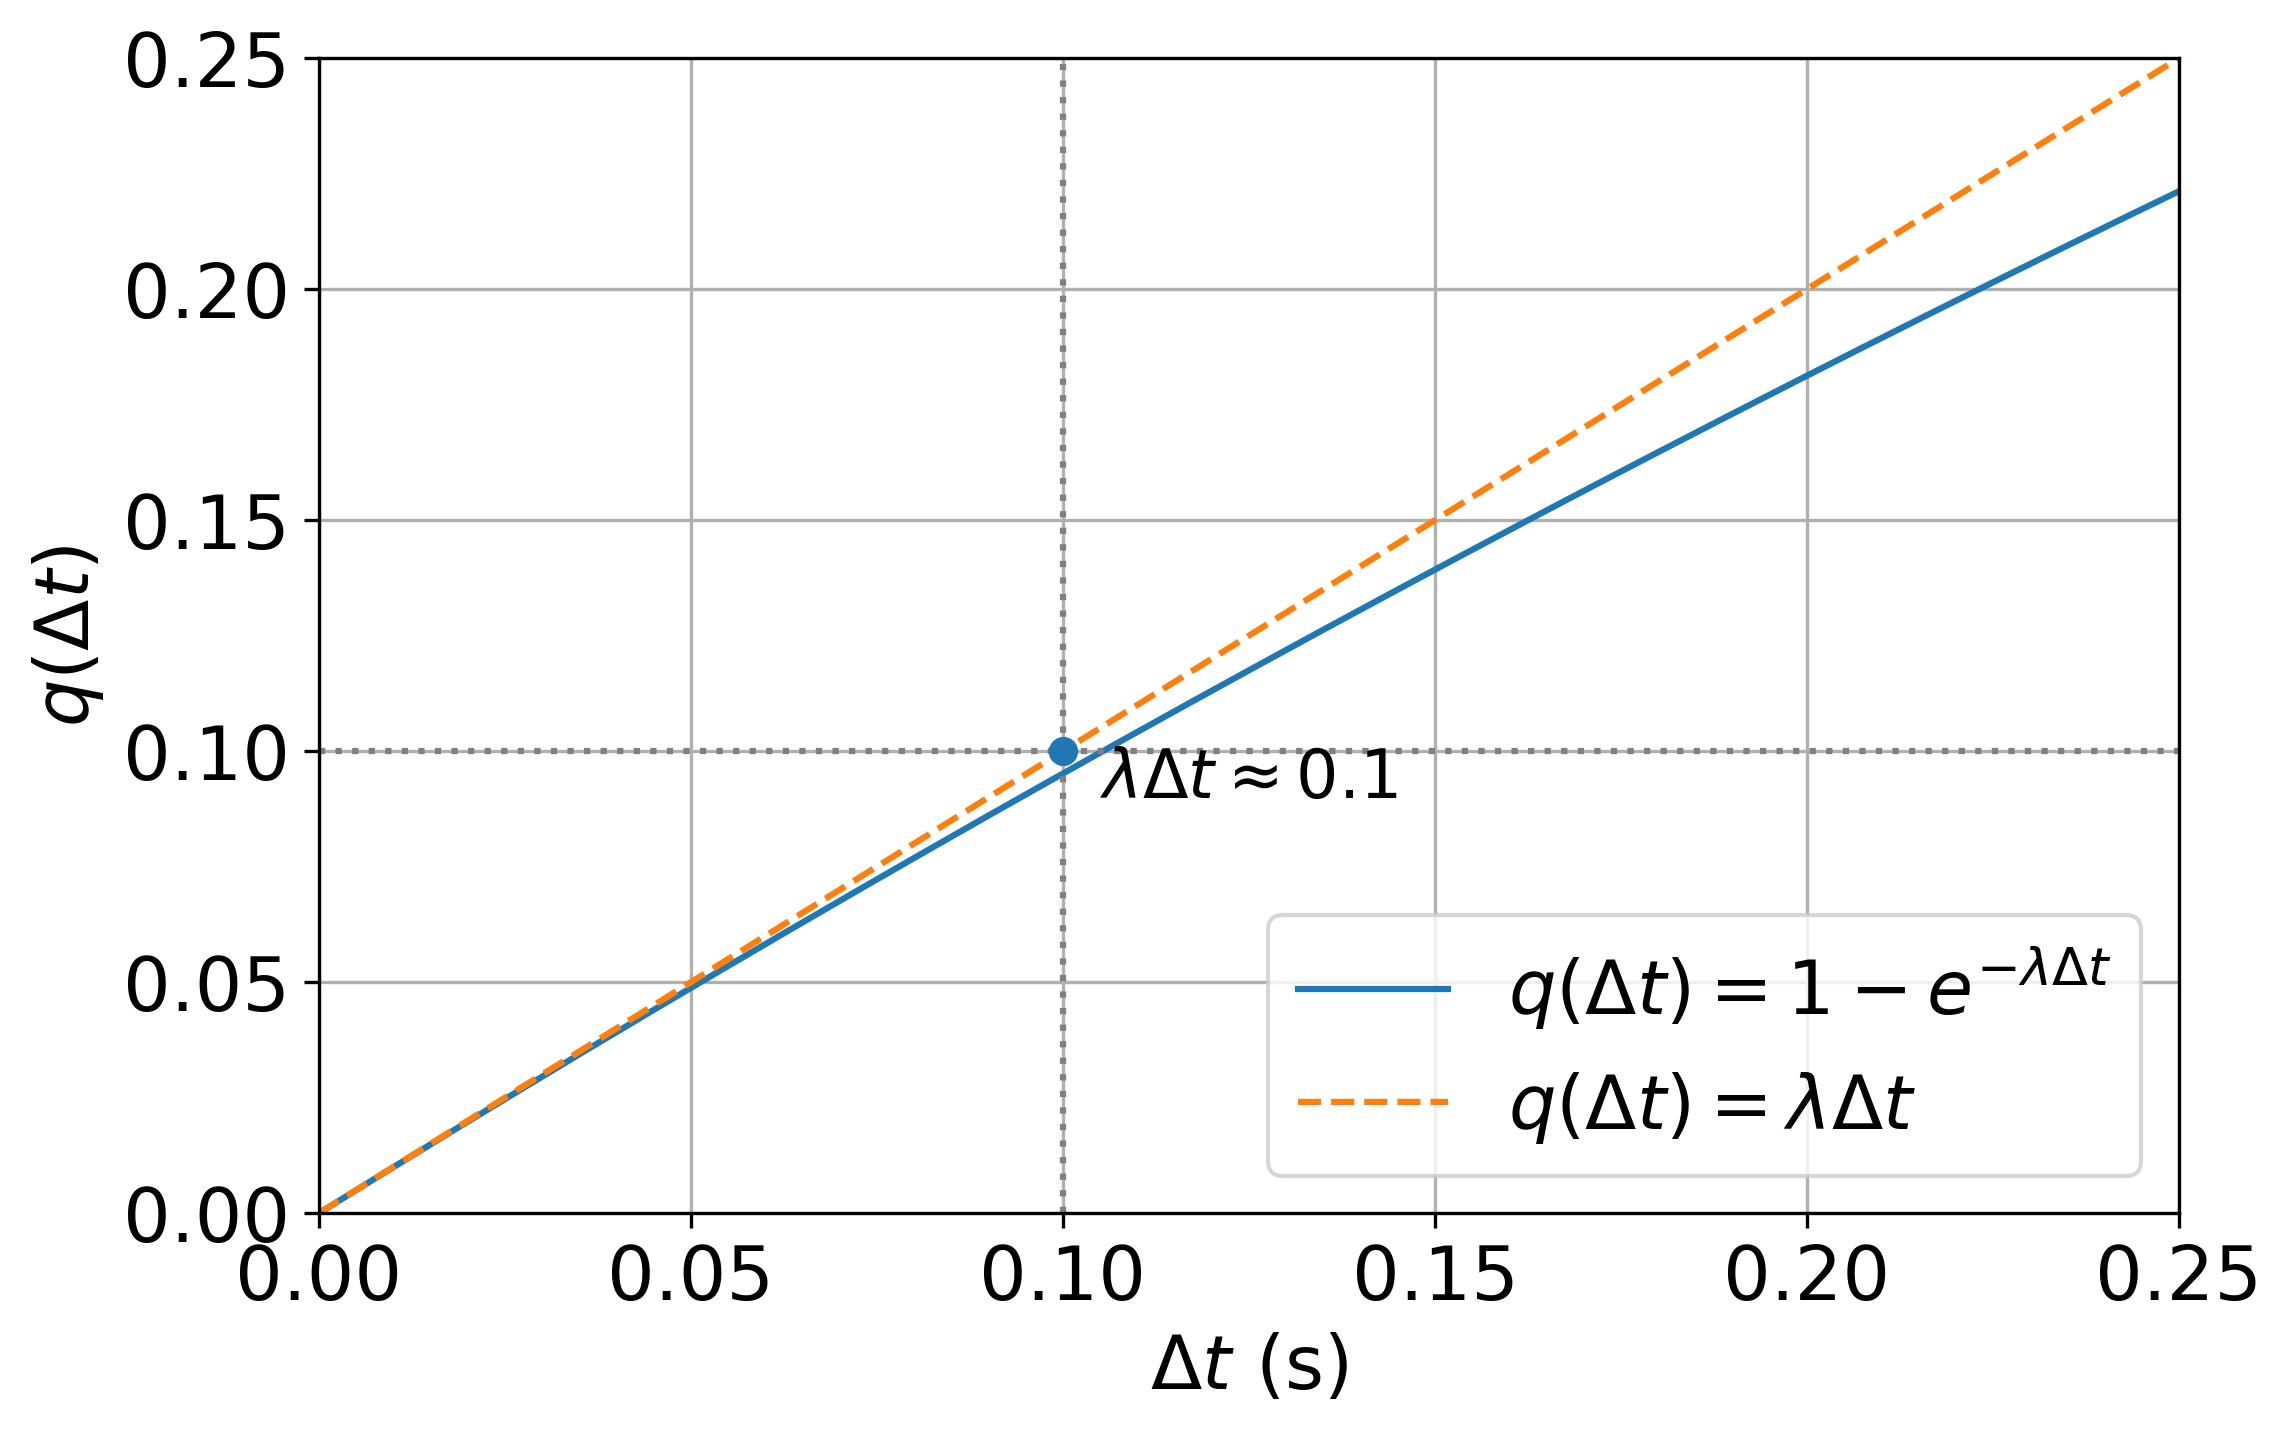
\includegraphics[width=1\textwidth]{Gráficas/exacta_vs_aprox.jpg}
    \caption{Probabilidad de desintegración exacta y aproximada}
    \label{fig:exacta_vs_aprox}
\end{figure}

La comparación muestra que la aproximación  $p \thickapprox  \lambda \Delta t$ es válida en el régimen $\lambda \Delta t \ll 1 $ donde la expansión de la exponencial a primer orden resulta adecuada.

\subsubsection{Distribuciones de probabilidad constante sin memoria}

En ciertos procesos físicos, como las desintegraciones radiactivas, la probabilidad de que ocurra un evento en un intervalo de tiempo no depende del tiempo previamente transcurrido. Este comportamiento se conoce como ausencia de memoria.

\begin{cajadefinicion}
Sea $X$ el tiempo hasta que ocurre un evento. Consideremos un instante $b$ tal que el evento no ha ocurrido todavía, es decir, $X>b$. En esta situación, nos interesa describir el tiempo restante hasta que ocurra el evento. \refmargen{Sheffield \cite{mit_poisson_notes}:}{Lecture 19, Memoryless ~~~~property}
Definimos la variable $Y = X - b$, que representa el tiempo restante hasta la ocurrencia del evento, condicionado a que $X > b$. Para cualquier valor $a$, se puede calcular

$$
P(Y > a \mid X > b),
$$

es decir,

$$
P(X - b > a \mid X > b) = P(X > b + a \mid X > b).
$$

Si $X$ sigue una distribución exponencial, se obtiene que

$$
P(X > b + a \mid X > b) = \frac{P(X > b + a)}{P(X > b)} = \frac{e^{-\lambda (b+a)}}{e^{-\lambda b}} = e^{-\lambda a}.
$$

Por tanto,

$$
P(Y > a \mid X > b) = P(X > a),
$$

lo que implica que la distribución del tiempo restante es la misma que la distribución original. Esta propiedad se conoce como ausencia de memoria. 
\end{cajadefinicion}

De hecho, la distribución exponencial es la única distribución continua que presenta la propiedad de ausencia de memoria, lo que explica su relevancia en la modelización de procesos físicos como las desintegraciones radiactivas.


\subsubsection{Densidad de probabilidad exponencial}
\begin{cajadefinicion} 
Sea $X$ una variable aleatoria. Decimos que $X$ es una variable contínua aleatoria si existe una función no negativa $f_X(x)$, definida para todos los reales $x\in [-\infty, \infty]$, con la propiedad de que para cualquier intervalo B de números reales \refmargen{Ross \cite{ross1993probabilitymodels}:}{\S~2.3}
\begin{equation}
  P\{X \in B\} = \int_B f_X(x)\,dx
  \label{eq:P(X in B)}
\end{equation}

siendo $f_X(x)$ la función densidad de probabilidad de la variable aleatoria $X$. 
\end{cajadefinicion}

La ecuación (\ref{eq:P(X in B)}) muestra que la probabilidad de que $X$ se encuentre en $B$ se puede obtener integrando la función densidad de probabilidad ``$f_X(x)$'' en ese intervalo.

Si $f_X(x)$ es evaluada en $[-\infty, \infty]$ debe satisfacer

\begin{equation}
  1= P \{X \in (-\infty, \infty) \} = \int_{-\infty}^{\infty} f_X(x)\,dx
\end{equation}

\begin{cajadefinicion}
  La densidad de probabilidad de desintegración $f_X(x)$ en su forma exponencial para la variable aleatoria $X$ con parámetro $\lambda$ \refmargen{Sheffield \cite{mit_poisson_notes}:}{Lecture 19; Exponential ~~~~~random variables}

\begin{equation}
f(x) =
\begin{cases}
\lambda e^{-\lambda x}, & x \geq 0 \\
0, & x < 0
\end{cases}
\label{eq:densidadpropexponencial}
\end{equation}

\end{cajadefinicion}

Considerando B como un intervalo cerrado $[0, b]$, entonces, si en (\ref{eq:P(X in B)}) introducimos (\ref{eq:densidadpropexponencial}): 

\begin{equation}
  \rightarrow P\{X \leq b\}=1-e^{-\lambda b} \label{eq:probabilidadintervalocerrado}
\end{equation}
\begin{equation}
  \rightarrow P\{X  > b\}=e^{-\lambda b}~~~~~
  \label{eq:probabilidadintervaloabierto}
\end{equation}

La ecuación (\ref{eq:probabilidadintervalocerrado}) es la probabilidad individual de que un núcleo se desintegre en un intervalo cerrado $[0, b]$, mientras qué, la ecuación (\ref{eq:probabilidadintervaloabierto}) es la probabilidad de que un núcleo individual no se haya desintegrado en ese mismo intervalo.

\begin{center}
  \textbf{SIGNIFICADO FÍSICO}
\end{center}

\begin{cajadefinicion}
  La densidad de probabilidad de desintegración $f(t)=\lambda e^{-\lambda t}$ describe como se distribuye en el tiempo la probabilidad de que un núcleo se desintegre, de modo que $f(t)dt$ representa la probabilidad de que la desintegración ocurra entre los instantes $t$ y $t+dt$.
\end{cajadefinicion}

\begin{figure}[H]
    \centering
    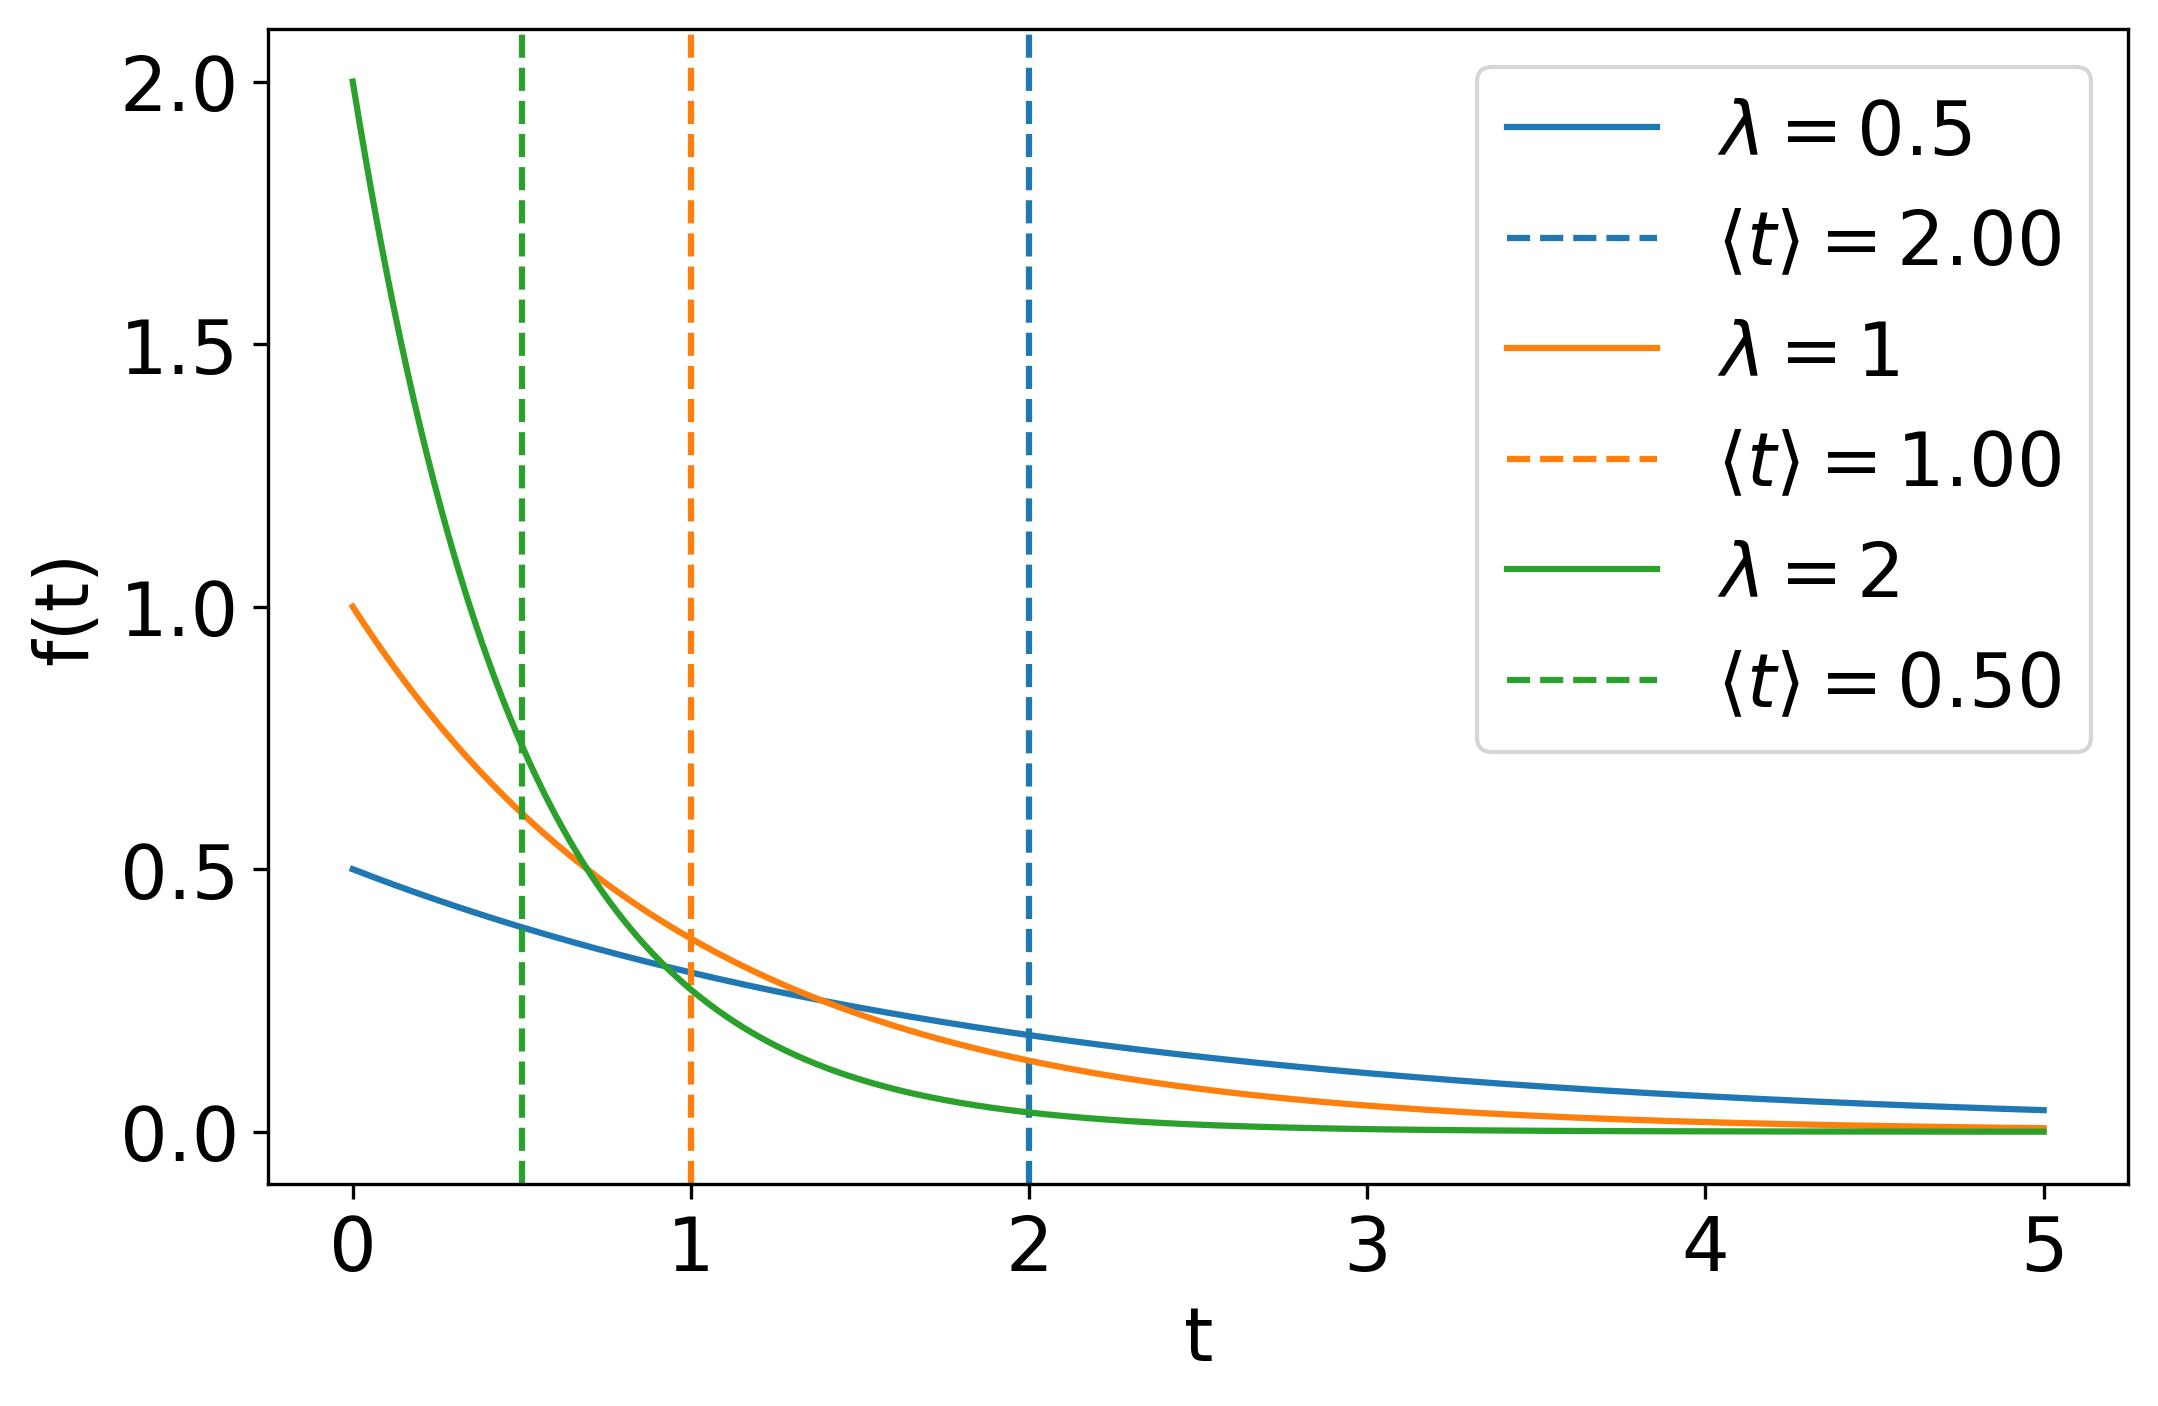
\includegraphics[width=1\textwidth]{Gráficas/f(t).jpg}
    \caption{Densidad de probabilidad de desintegración para distintos valores de $\lambda$. Las líneas discontinuas indican el valor medio $\langle t \rangle = 1/\lambda$.}
    \label{fig:densidadpropexponencial}
\end{figure}

\begin{itemize}
  \item $f(t)$ tiene un máximo en $t=0$ con valor $\lambda$, la constante de desintegración. Esto indica que la probabilidad instantánea de desintegración es máxima al inicio. Sin embargo, debido al carácter sin memoria del proceso, esta tasa de desintegración permanece constante en todo instante, siendo $\lambda$ la probabilidad por unidad de tiempo de desintegración para un núcleo que ha sobrevivido hasta ese momento.
  \item Tiempo medio 
  \begin{equation}
     \langle t \rangle = \int_{0}^{\infty} t \lambda e^{-\lambda t} \,dt = \frac{1}{\lambda}
  \end{equation}
  \item Varianza 
  \begin{equation}
    \sigma^2 = \int_{0}^{\infty} (t-\langle t \rangle)^2 \lambda e^{-\lambda t} \,dt = \frac{1}{\lambda^2}
  \end{equation}
  \item Desviación típica 
  \begin{equation}
    \sigma = \sqrt{\sigma^2} = \frac{1}{\lambda}
  \end{equation}
\end{itemize}

\subsubsection{Ley de probabilidad de supervivencia}
Uno de los requisitos para entender las desintegraciones radiactivas, es conocer la ley de probabilidad de supervivencia $S(t)$. Esta nos permitirá describir el comportamiento de las desintegraciones radiactivas en el tiempo.

La probabilidad de supervivencia de un núcleo en un tiempo $t$ es (\ref{eq:probabilidadintervaloabierto}):


\begin{equation}
  p(t) = P\{X > t\} = e^{-\lambda t}
\end{equation}

Si consideramos un intervalo de tiempo infinitesimal $dt$, la probabilidad de supervivencia de un núcleo en el intervalo $[t, t+dt]$ es

$$
  p(dt)= P\{X > t + dt \mid X > t\} = \frac{P\{X > t + dt\}}{P\{X > t\}} = \frac{e^{-\lambda (t+dt)}}{e^{-\lambda t}} = e^{-\lambda dt} 
$$

\begin{equation}
  p(dt) \approx 1 - \lambda dt
  \label{eq:probabilidaddesupervivenciaintervalodt}
\end{equation}

De esta manera, podemos derivar la ley de probabilidad de supervivencia $S(t)$ a partir de su forma discreta:

$$
  S(t+dt) = S(t)(1-\lambda dt)  \rightarrow S(t+dt)-S(t)=-S(t)\lambda dt
$$

Tomándo el límite en $dt \rightarrow 0$:

$$
  \lim_{dt \rightarrow 0} \frac{S(t+dt) - S(t)}{dt}  = \lim_{dt \rightarrow 0} -S(t)\lambda
$$

Obtenemos:

\begin{equation}
  \frac{dS}{dt}= -\lambda S
  \label{eq:diferencial_leysupervivencia}
\end{equation}

Llegando finalmente a la ley de probabilidad de supervivencia(función de supervivencia):
\begin{equation}
  S(t) = e^{-\lambda t}
\end{equation}

En relación con la función densidad de propabiblidad (\ref{eq:densidadpropexponencial}):

\begin{cajadefinicion}
  La función de supervivencia $S(t)$, definida como la probabilidad de que el núcleo no se haya desintegrado hasta el instante $t$, puede expresarse como \refmargen{Lawless \cite{lawless2011lifetime}: }{eq 1.2.1}

\begin{equation}
  S(t) = P(T \geq t) = \int_t ^{\infty} f(t)\,dt
  \label{eq:defsupervivencia}
\end{equation}

\end{cajadefinicion}

$S(t)$ es una función contínua monótona decreciente con $S(0) = 1$, es decir, el máximo de la función densidad de probabilidad ($t=0$) en el caso de un núcleo se traduce a que lo más probable es que se desintegre lo antes posible; y $lim_{t \rightarrow \infty} S(t) = 0$. Algunas veces se debe considerar $S(\infty)>0$ pues algunos núcleos nunca decaen.

De la ecuación que define la ley de supervivencia (\ref{eq:defsupervivencia}), se obtiene la relación:

\begin{equation}
  f(t)=-\frac{dS(t)}{dt}
\end{equation}

\subsubsection{Ley de desintegración radiactiva}

Como consecuencia de la hipótesis fundametal, si $N$ núcleos radiactivos están presentes a tiempo t y no se introducen nuevos,  entonces el número de  núcleos decayendo en un tiempo $dt$, $dN$, es proporcional a $N$.  \refmargen{Krane \cite{krane}:}{\S~6.1}

\begin{equation}
\frac{dN}{dt} = - \lambda N
\label{eq:desintegración}
\end{equation}

Esta ecuación es, en realidad, la forma diferencial de la ley de supervivencia (\ref{eq:diferencial_leysupervivencia}) empleando la variable aleatoria $N(t)$(número de núcleos a tiempo t). 

De la ecuación (\ref{eq:desintegración}) llegamos a:

\begin{equation}
N(t) = N_0 e^{-\lambda t}
\label{eq:ley_desintegracion}
\end{equation}

Lo que nos permite obtener:

\begin{equation}
  t = \frac{1}{\lambda} \ln(\frac{N_0}{N})
  \label{eq:tiempo_estimado}
\end{equation}

\subsubsection{Magnitudes resultantes de la ley de desintegración radiactiva}

La \textbf{semivida} es el tiempo necesario para que se desintegren la mitad de los núcleos de una muestra y está relacionada con la constante de desintegración $\lambda$ mediante la ecuación:

\begin{equation}
t_{1/2} = \frac{\ln2}{\lambda}
\label{eq:half-life}
\end{equation}

El \textbf{tiempo medio de vida} de un núcleo es:

\begin{equation}
\tau = \frac{\int_{0}^{\infty} t|dN/dt| \,dt }{\int_{0}^{\infty} |dN/dt|\,dt}
\end{equation}

Resolviendo:

\begin{equation}
\tau = \frac{\int_{0}^{\infty} t|dN/dt| \,dt }{N_0} = \frac{\lambda \int_{0}^{\infty} t N_0 e^{-\lambda t} \,dt}{N_0} = \frac{\lambda}{\lambda^2}= \frac{1}{\lambda}
\end{equation}

Es decir que el tiempo medio de vida de un núcleo es la inversa de la constante de desintegración.

La \textbf{actividad} es el número de desintegraciones radiactivas por unidad de tiempo:

\begin{equation}
A = \lambda N(t) = \lambda N_0 e^{-\lambda t} = A_0 e^{-\lambda t}
\label{eq:activity}
\end{equation}

Obtener el número de núcleos en un tiempo $t$ es bastante complidado si $\lambda$ no es conocido. Sin embargo, sí se puede medir la radiación emitida por una fuente en un intervalo de tiempo $t$, es decir, el número de desintegraciones que tienen lugar en dicho intervalo:

\begin{equation}
|\Delta N| = N(t) - N(t + \Delta t) = N_0 e^{-\lambda t}(1-e^{-\lambda \Delta t})
\end{equation}

Esta magnitud está directamente relacionada con la actividad (\ref{eq:activity}) de la muestra, lo que permite acceder experimentalmente a la constante de desintegración $\lambda$.


\subsection{Descripción estadística de una muestra radiactiva}
La ley de desintegración obtenida (\ref{eq:desintegración}) no describe un proceso determinista, es un comportamiento promedio.

Partiendo de $N_0$ núcleos independientes, cada núcleo individual tiene una probabilidad $q(t)= 1-e^{-\lambda t}$ de desintegrarse en un intervalo de tiempo $[0,t]$ (\ref{eq:probabilidadintervalocerrado}). El resto de núcleos que no se desintegran se almacenan en la variable aleatoria $N(t)$,  la cual sigue la \textbf{distribución binomial} (\ref{eq:distribucionbinomial}):

\subsubsection{Distribución Binomial}

Para llegar a la distribución binomial, se escoge un sistema físico que muestre dos resultados posibles, como por ejemplo el lanzamiento de una moneda. Partiendo de 5 monedas, a cada moneda se le asigna una letra A, B, C, D y E. El objetivo es obtener 3 monedas cara. Sean A, B y C cara y D y E cruz. Al escoger la primera moneda, puede estar en 5 posiciones distintas, la siguiente moneda puede estar en 4 posiciones distintas y la tercera en 3 posiciones. Por lo tanto($5\cdot 4\cdot 3$), existen 60 permutaciones posibles de escoger A, B y C.

Como el objetivo es obtener 3 monedas cara, el orden en el que se escojan las monedas no importa, por lo que se debe dividir entre el número de combinaciones posibles de las monedas cara, es decir, 6 ($3\cdot 2\cdot 1$). De esta manera, se obtiene que existen 10 combinaciones distintas de obtener 3 monedas cara. Matemáticamente:

$$\binom{5}{3} = \frac{60}{6} = 10$$

Esto se conoce como el \textbf{Coeficiente Binomial}. \refmargen{Bevington \cite{bevington}: }{\S~2.1}

\begin{cajadefinicion}
  Sea $n$ el número de ensayos independientes, $x$ el número de éxitos. El número de permutaciones posibles de obtener $x$ éxitos en $n$ ensayos es:
  $$P_m=n(n-1)(n-2)...(n-x+1)=\frac{n!}{(n-x)!}$$
  
  No obstante, $x$ combinaciones de éxitos se pueden ordenar de $x!$ formas distintas, por lo que el número de combinaciones posibles de obtener $x$ éxitos en $n$ ensayos es el  \textbf{coeficiente binomial} C(n,x):
  \begin{equation}
    C(n,x) = \binom{n}{x} = \frac{P_m}{x!} = \frac{n!}{x!(n-x)!}
  \end{equation}
\end{cajadefinicion}

Para obtener la probabilidad de conseguir $x$ éxitos en $n$ ensayos ($P(n,x)$) se debe multiplicar $C(n,x)$ por la probabilidad individual de que salga cierto resultado.

La probabilidad de obtener $x$ éxitos es $p^x$ siendo $p$ la probabilidad de éxito en un ensayo. La probabilidad de obtener $n-x$ fracasos es $q^{n-x}=(1-p)^{n-x}$. Finalmente llegamos a la probabilidad de la \textbf{distribución binomial}:

\begin{equation}
  P(n,x) = C(n,x) p^x q^{n-x} = \binom{n}{x} p^x (1-p)^{n-x}
  \label{eq:distribucionbinomial}
\end{equation}

\subsubsection{Media de la Distribución Binomial}

La media o valor esperado de una variable aleatoria binomial $X\sim B(n,p)$ se define como:

\begin{equation}
    \mu = \sum_{x=0}^{n} x P(X=x) = \sum_{x=0}^{n} x\frac{n!}{x!(n-x)!} p^x(1-p)^{n-x} \refmargen{Bevington \cite{bevington}: }{eq~2.6}
\end{equation}

El término correspondiente a $x=0$ no contribuye a la suma, ya que queda multiplicado por cero. Por tanto, se puede escribir:

\begin{equation}
    \mu = \sum_{x=1}^{n} x\frac{n!}{x!(n-x)!}p^x(1-p)^{n-x}
  \label{eq:mediabinomial}
\end{equation}



Como $x! = x(x-1)!$, se tiene:

$$
    x\binom{n}{x}
    =
    \frac{n!}{x!(n-x)!}
    =
    x\frac{n!}{x(x-1)!(n-x)!}
$$

Cancelando el factor $x$:

$$
    x\binom{n}{x}
    =
    \frac{n!}{(x-1)!(n-x)!}
$$

Además, como $n! = n(n-1)!$, queda:

$$
    x\binom{n}{x}
    =
    n\frac{(n-1)!}{(x-1)!(n-x)!}
$$

Esta expresión puede escribirse como:

$$
    x\binom{n}{x}
    =
    n\binom{n-1}{x-1}
$$

Sustituyendo este resultado en la expresión de la media (\ref{eq:mediabinomial}):

\begin{equation}
    \mu =
    \sum_{x=1}^{n}
    n\binom{n-1}{x-1}p^x(1-p)^{n-x}
\end{equation}

Como $n$ no depende del índice de la suma, puede sacarse fuera:

$$
    \mu =
    n\sum_{x=1}^{n}
    \binom{n-1}{x-1}p^x(1-p)^{n-x}
$$

Ahora se separa un factor $p$, usando que $p^x=p\,p^{x-1}$:

$$
    \mu =
    np\sum_{x=1}^{n}
    \binom{n-1}{x-1}p^{x-1}(1-p)^{n-x}
$$

Se realiza el cambio de variable:

\begin{equation}
    y=x-1
\end{equation}

Cuando $x=1$, entonces $y=0$, y cuando $x=n$, entonces $y=n-1$. Además:

$$
    x-1=y,
    \qquad
    n-x=n-1-y
$$

Por tanto, la suma queda:

\begin{equation}
    \mu =
    np\sum_{y=0}^{n-1}
    \binom{n-1}{y}p^y(1-p)^{n-1-y}
\end{equation}

La suma que aparece es la suma de todas las probabilidades de una distribución binomial con $n-1$ ensayos, por lo que vale 1. Empleando el binomio de Newton:

$$
    \sum_{y=0}^{n-1}
    \binom{n-1}{y}p^y(1-p)^{n-1-y}
    =
    \left[p+(1-p)\right]^{n-1}
    =
    1^{n-1}
    =
    1
$$

Por tanto, la \textbf{media de una distribución binomial} es:

\begin{equation}
    \boxed{\mu = np}
    \label{eq:media_distribucion_binomial}
\end{equation}

\subsubsection{Varianza y desviación típica de una distribución binomial}

La varianza de una variable aleatoria $X$ puede escribirse como:

\begin{equation}
    \sigma^2 = E[X^2]-\mu^2
    \label{eq:varianza}
\end{equation}

donde $\mu=E[X]$. Para una distribución binomial $X\sim B(n,p)$, ya se ha obtenido que $\mu = np$, por tanto, para calcular la varianza es necesario obtener primero $E[X^2]$. Por definición:

\begin{equation}
    E[X^2]
    =
    \sum_{x=0}^{n}
    x^2
    \binom{n}{x}
    p^x(1-p)^{n-x}
\end{equation}

Para simplificar esta suma, se utiliza la identidad:

\begin{equation}
    x^2=x(x-1)+x
\end{equation}

Así:

$$
    E[X^2]
    =
    E[X(X-1)]+E[X]
$$

Como $E[X]=\mu=np$, queda:

$$
    E[X^2]
    =
    E[X(X-1)]+np
$$

Calculamos ahora $E[X(X-1)]$:

\begin{equation}
    E[X(X-1)]
    =
    \sum_{x=0}^{n}
    x(x-1)
    \binom{n}{x}
    p^x(1-p)^{n-x}
\end{equation}

Los términos $x=0$ y $x=1$ no contribuyen, ya que $x(x-1)=0$. Por tanto:

\begin{equation}
    E[X(X-1)]
    =
    \sum_{x=2}^{n}
    x(x-1)
    \binom{n}{x}
    p^x(1-p)^{n-x}
\end{equation}

Se desarrolla ahora el factor $x(x-1)\binom{n}{x}$:

$$
    x(x-1)\binom{n}{x}
    =
    x(x-1)\frac{n!}{x!(n-x)!}
$$

Como:

$$
    x! = x(x-1)(x-2)!
$$

entonces:

$$
    x(x-1)\binom{n}{x}
    =
    x(x-1)
    \frac{n!}{x(x-1)(x-2)!(n-x)!}.
$$

Cancelando el factor $x(x-1)$:

$$
    x(x-1)\binom{n}{x}
    =
    \frac{n!}{(x-2)!(n-x)!}
$$

Además, como:

$$
    n! = n(n-1)(n-2)!
$$

se obtiene:

\begin{equation}
    x(x-1)\binom{n}{x}
    =
    n(n-1)
    \frac{(n-2)!}{(x-2)!(n-x)!}
\end{equation}

Esta expresión puede escribirse como:

\begin{equation}
    x(x-1)\binom{n}{x}
    =
    n(n-1)\binom{n-2}{x-2}
\end{equation}

Sustituyendo en la suma:

\begin{equation}
    E[X(X-1)]
    =
    \sum_{x=2}^{n}
    n(n-1)
    \binom{n-2}{x-2}
    p^x(1-p)^{n-x}
\end{equation}

Como $n(n-1)$ no depende del índice de la suma, puede sacarse fuera:

$$
    E[X(X-1)]
    =
    n(n-1)
    \sum_{x=2}^{n}
    \binom{n-2}{x-2}
    p^x(1-p)^{n-x}
$$

Ahora se separa un factor $p^2$, usando que $p^x=p^2p^{x-2}$:

$$
    E[X(X-1)]
    =
    n(n-1)p^2
    \sum_{x=2}^{n}
    \binom{n-2}{x-2}
    p^{x-2}(1-p)^{n-x}
$$


Se realiza el cambio de variable:

\begin{equation}
    y=x-2
\end{equation}

Cuando $x=2$, entonces $y=0$, y cuando $x=n$, entonces $y=n-2$. Además:

$$
    x-2=y,
    \qquad
    n-x=n-2-y
$$

Por tanto:

\begin{equation}
    E[X(X-1)]
    =
    n(n-1)p^2
    \sum_{y=0}^{n-2}
    \binom{n-2}{y}
    p^y(1-p)^{n-2-y}.
\end{equation}

La suma que aparece es la suma de todas las probabilidades de una distribución binomial con $n-2$ ensayos, por lo que vale 1. Empleando el binomio de Newton:

$$
    \sum_{y=0}^{n-2}
    \binom{n-2}{y}
    p^y(1-p)^{n-2-y}
    =
    [p+(1-p)]^{n-2}
    =
    1^{n-2}
    =
    1
$$

Así:

$$
    E[X(X-1)] = n(n-1)p^2.
$$

Por tanto:

\begin{equation}
    E[X^2]
    =
    E[X(X-1)]+E[X]
    =
    n(n-1)p^2+np
\end{equation}

Finalmente, usando la expresión de la varianza(\ref{eq:varianza}) y sabiendo que $\mu=np$, se obtiene:

$$
    \sigma^2
    =
    n(n-1)p^2+np-(np)^2
      =
    np-np^2
$$

Sacando factor común $np$ llegamos a la \textbf{varianza de la distribución binomial}:

\begin{equation}
    \boxed{Var=\sigma^2=np(1-p)}
\end{equation}

Y la \textbf{desviación típica de la distribución binomial} es:
\begin{equation}
    \boxed{\sigma = \sqrt{Var} = \sqrt{np(1-p)}}
     \label{eq:desviación_típica_binomial}
\end{equation}

%%%%% TENGO QUE DEMOSTRAR QUE PARA UN INTERVALO 


\subsubsection{Aproximación de Poisson}

Cuando el número inicial de núcleos $N_0$ es grande y la probabilidad de desintegración en el intervalo $[0,t]$ es pequeña, es decir, $t$ es pequeño comparado con la vida media, la distribución binomial se aproxima a la \textbf{distribución de Poisson}. Concretamente para el número de núcleos desintegrados en el intervalo $[0,t]$

\begin{equation}
  D(t)=N_0-N(t)
  \label{eq:núcleosdesintegrados}
\end{equation}

se tiene que

\begin{equation}
  P(D(t)=n)\approx \frac{(\mu)^n}{n!} e^{-\mu},~~~~~~~\mu= N_0(1-e^{-\lambda t}) \approx N_0\lambda t
  \label{eq:poisson}
\end{equation}

\begin{cajadefinicion}
  Un proceso de Poisson, con tasa $\lambda$, es un proceso $N=\{ N(t):t \geq 0 \}$ que toma valores en $S=\{ 0,1,2,... \}$ tal que:
  \begin{enumerate}
    \item Comienza en 0:$N(0)=0$ 
    \item No decrece: $N(s) \leq N(t)$ si $s < t$
    \item Si $s < t$, el número de emisiones $N(t)-N(s)$ en un intervalo $(s,t]$ no afecta a lo que ocurre en otro intervalo $[0,s]$ que no se solapa. \refmargen{Grimmett \cite{grimmett2020probability}:}{\S~6.8}
    \item En un intervalo muy pequeño de duración $h$ , la probabilidad de que ocurra exactamente una desintegración es aproximadamente $\lambda h$, la probabilidad de que ocurra más de una es prácticamente cero ($o(h)$), y la probabilidad de que no ocurra ninguna es $1 - \lambda h + o(h)$.
  \end{enumerate}
  \label{def:procesodepoisson}
\end{cajadefinicion}

El proceso de Poisson solo es válido para intervalos cortos. Conforme el tiempo avanza, el número de núcleos que quedan se reduce y la tasa de desintegración deja de ser constante, quitándole el carácter de homogeneidad al proceso de Poisson.

\subsection{Valor esperado de la distribución de Poisson, Varianza y Desviación típica}

\subsection{Técnica de Montecarlo}

% --------------------------------------------------

\section{Metodología}

\subsection{Simulaciones iniciales}
Antes de comenzar con la datación radiométrica, es necesario escoger un modelo de simulación que permita describir el proceso de desintegración radiactiva. Para ello, se han elegido tres modelos de simulación distintos que emplean la técnica o modelo de Monte Carlo.


De cara a estas primeras simulaciones, se ha empleado los valores para la constante de desintegración $\lambda = 1$, el número inicial de núcleos $N_0 = 1000$, un tiempo total de simulación $t=5$ años, suficiente para que se desintegren todos los núcleos y un intervalo de tiempo $dt=0.05$ años.

%%% TENGO QUE MOSTRAR QUE LAS SIMULACIONES SON ÚNICAS


\subsubsection{Simulación núcleo a núcleo}
En este modelo se representa explícitamente cada uno de los núcleos iniciales $N_0$. El tiempo total de la simulación se divide en intervalos de duración $dt$. A cada núcleo se le asigna una probabilidad de desintegración
  
\begin{equation}
  q = 1 - e^{-\lambda dt}
  \label{eq:probabilidad_desintegración}
\end{equation}

Con el fin de conocer el destino de cada núcleo, se genera un número aleatorio ``$r$'' para cada uno de ellos, el cual estará uniformemente distribuido entre 0 y 1, \refmargen{Hauf2013 \cite{Hauf2013}}{\S~III.B}. Si el número aleatorio generado es menor que la probabilidad de desintegración ($r < q$), se considmera que ese núcleo se ha desintegrado, en caso contrario, el núcleo sobrevivirá. Este proceso se repite para cada núcleo presente en cada intervalo de tiempo $dt$ hasta alcanzar el tiempo total de simulación $t$. 

\begin{figure}[H]
  \centering
  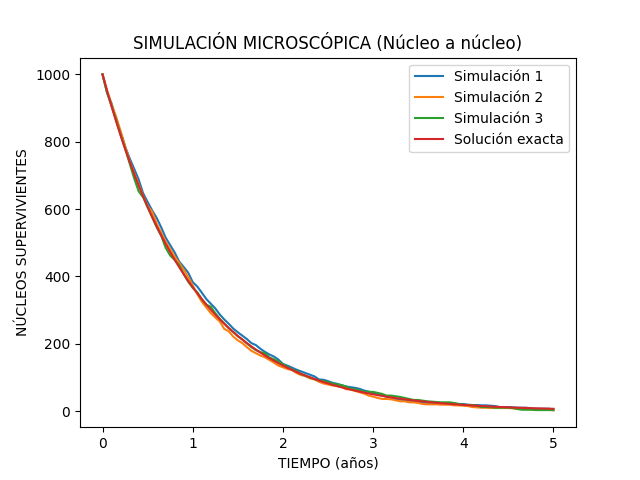
\includegraphics[width=1\textwidth]{TAREA2/microscopic.png}
  \caption{3 simulaciones realizadas con el modelo microscópico núcleo a núcleo.}
\end{figure}

\subsubsection{Simulación con distribución binomial}
Este modelo no simula individualmente el destino de cada núcleo, sino que se genera directametne el número de núcleos que se desintegran en cada intervalo de tiempo $dt$. Al inicio de cada intervalo, se conoce el número de núcleos supervivientes $N_i$, siendo la probabilidad de supervivencia de cada uno de ellos

\begin{equation}
  p = e^{-\lambda dt}
  \label{eq:probabilidad_supervivencia}
\end{equation}

El número de núcleos supervivientes al final del intervalo, queda determinado mediante una distribución binomial con parámetros $N_i$ y $p$  (\ref{eq:distribucionbinomial}). 

\begin{equation}
N_{i+1} \sim \operatorname{Bin}(N_i,p)
\end{equation}

De esta forma, se genera un único número aleatorio para cada paso temporal, el cual, representa el número de núcleos supervivientes al final del intervalo. Es decir, estes valor se emplea como población incial al comienzo del siguiente intervalo. Este proceso se repite hasta alcanzar el tiempo total de simulación $t$.

\begin{figure}[H]
  \centering
  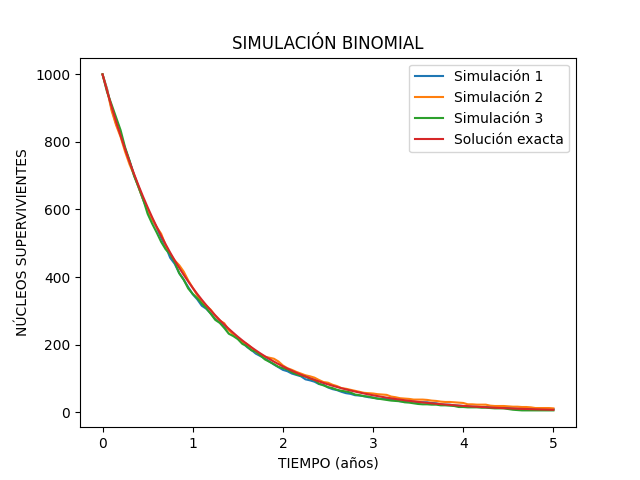
\includegraphics[width=1\textwidth]{TAREA2/binomial.png}
  \caption{3 simulaciones realizadas con la modelo de distribución binomial.}
\end{figure}

\subsubsection{Simulación con aproximación de Poisson}
Cuando la probabilidad de desintegración durante el intervalo es pequeña, se puede conocer el número de núcleos desintegrados aproximando la distribución binomial a la distribución de Poisson (\ref{eq:poisson}).

\begin{equation}
D_i\sim\operatorname{Poi}(\mu_i).
\end{equation}

donde $\mu_i = N_i(1-e^{-\lambda dt})$ es el número medio de núcleos que se desintegran en el intervalo $[t_i, t_i + dt]$.

Una vez generado el número de desintegraciones, la población de núcleos supervivientes se actualiza según

\begin{equation}
N_{i+1}=N_i-D_i.
\end{equation}

De esta forma, en cada paso temporal se genera un único número aleatorio que representa el número total de núcleos desintegrados. La tasa media se recalcula a partir de la población presente $N_i$, y el proceso se repite hasta alcanzar el tiempo total de simulación $t$.

\begin{figure}[H]
  \centering
  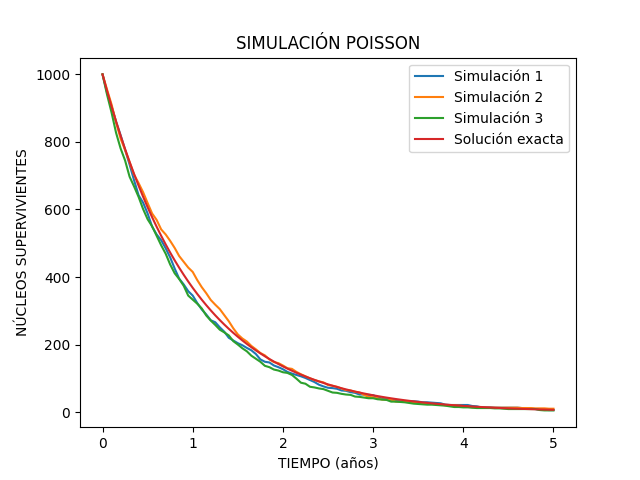
\includegraphics[width=1\textwidth]{TAREA2/poisson.png}
  \caption{3 simulaciones realizadas con la aproximación de Poisson.}
\end{figure}

\subsubsection{Comparación de los modelos de simulación}

\begin{figure}[H]
  \centering
  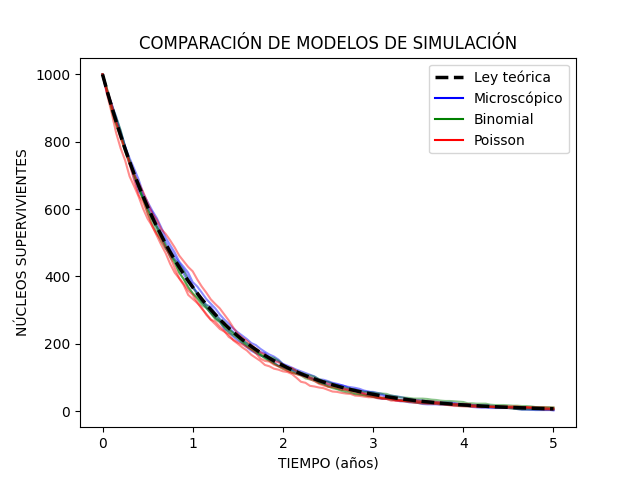
\includegraphics[width=1\textwidth]{TAREA2/comparacion.png}
  \caption{Comparación de las 3 simulaciones de cada modelo frente a la solución exacta.}
\end{figure}

El modelo núcleo a núcleo y el modelo binomial muestran el mismo comportamiento estadístico, aunque difieren en la forma de simular el proceso. Esto permite descartar uno de ellos y conservar únicamente el modelo binomial, ya que realiza menos de 1000 operaciones por simulación, mientras que el modelo núcleo a núcleo puede requerir decenas de miles. Esta diferencia también se refleja en el tiempo de ejecución, que resulta notablemente mayor para el modelo núcleo a núcleo.

La aproximación de la distribución binomial a la distribución de Poisson es una buena aproximación para intervalos cortos y muchos núcleos. En este caso, 1000 núcleos y un intervalo de 0.05, la aproximación es notablemente buena. No obstante, esta aproximación pierde precisión a medida que aumente el intervalo temporal, ya que también crece la probabilidad de desintegración en cada paso (\ref{eq:probabilidad_desintegración}).
La distribución binomial y de poisson presentan el mismo valor esperado pero no la misma varianza. La varianza de la distribución binomial es $np(1-p)$, mientras que la de la distribución de Poisson es $n p$. En este caso, con un paso de 0.05, el factor $1-p\approx 1$. A partir del $10\%$ de diferencia entre varianzas

$$1-\frac{Var_{Bin}}{Var_{Poi}} \thickapprox 10\%$$

la aproximación de la distribución binomial a la distribución de Poisson comienza a perder precisión.

Para un intervalo de 0.2 años y 1000 núcleos.

\begin{figure}[H]
  \centering
  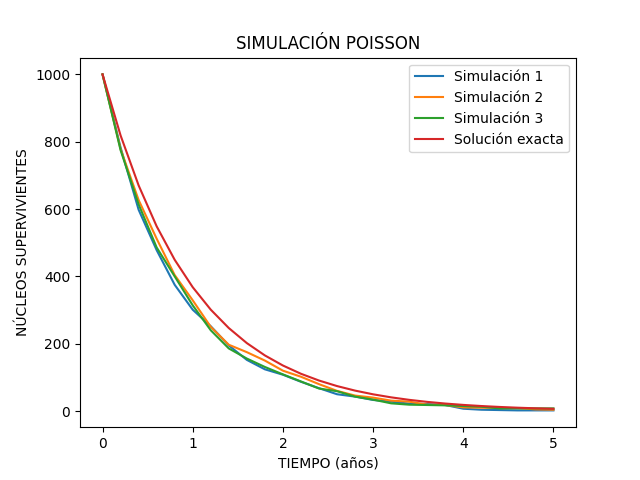
\includegraphics[width=1\textwidth]{TAREA2/0.2poisson.png}
  \caption{3 simulaciones realizadas con la aproximación de Poisson para un paso de 0.2 años.}
\end{figure}

Para el caso de pocos núcleos, 100 núcleos, manteniendo el paso de 0.05 años, el valor esperado $\mu = np \thickapprox 5$. Es decir, por intervalo de tiempo, se desintegran solo 5 núcleos, haciendo las estadística muy pobre.

\begin{figure}[H]
  \centering
  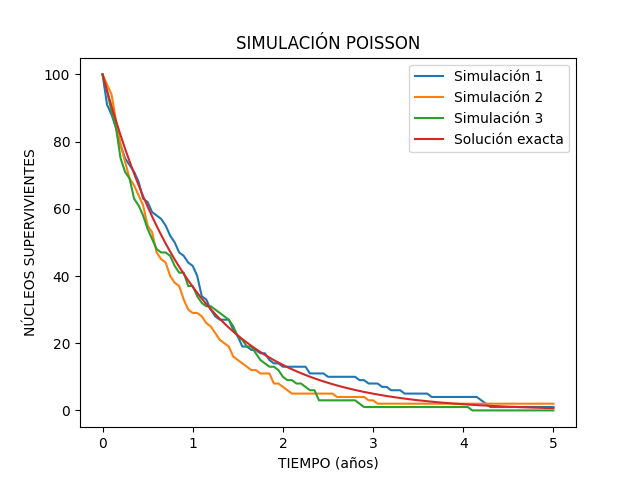
\includegraphics[width=1\textwidth]{TAREA2/100poisson.png}
  \caption{3 simulaciones realizadas con la aproximación de poisson para un paso de 0.05 años y 100 núcleos.}
\end{figure}

\subsection{Validación estadística del modelo binomial}

Una vez seleccionado el modelo binomial como modelo de simulación, se debe comprobar si reproduce correctamente la ley macroscópica de desintegración radiactiva. Para ello, se repite la simulación $M=50$ veces, manteniendo fijos los parámetros $N_0$, $\lambda$, $dt$ y el tiempo total de simulación. Cada repetición representa una posible trayectoria temporal del número de núcleos supervivientes.

A partir de estas $M$ simulaciones se calcula, para cada instante temporal ($t_i$), el valor medio del número de núcleos supervivientes,

\begin{equation}
\overline{N}_i=\frac{1}{M}\sum_{j=1}^{M}N_i^{(j)}.
\label{eq:valor_medio_Msimulaciones}
\end{equation}

así como la desviación típica asociada,

\begin{equation}
\sigma_i=
\sqrt{
\frac{1}{M-1}
\sum_{j=1}^{M}
\left(N_i^{(j)}-\overline{N}_i\right)^2
}.
\label{eq:desviación_típica_Msimulaciones}
\end{equation}

De esta forma, se puede comparar el comportamiento promedio de la simulación con la ley teórica de desintegración,

$$
N(t)=N_0e^{-\lambda t}.
$$

\begin{figure}[H]
\centering
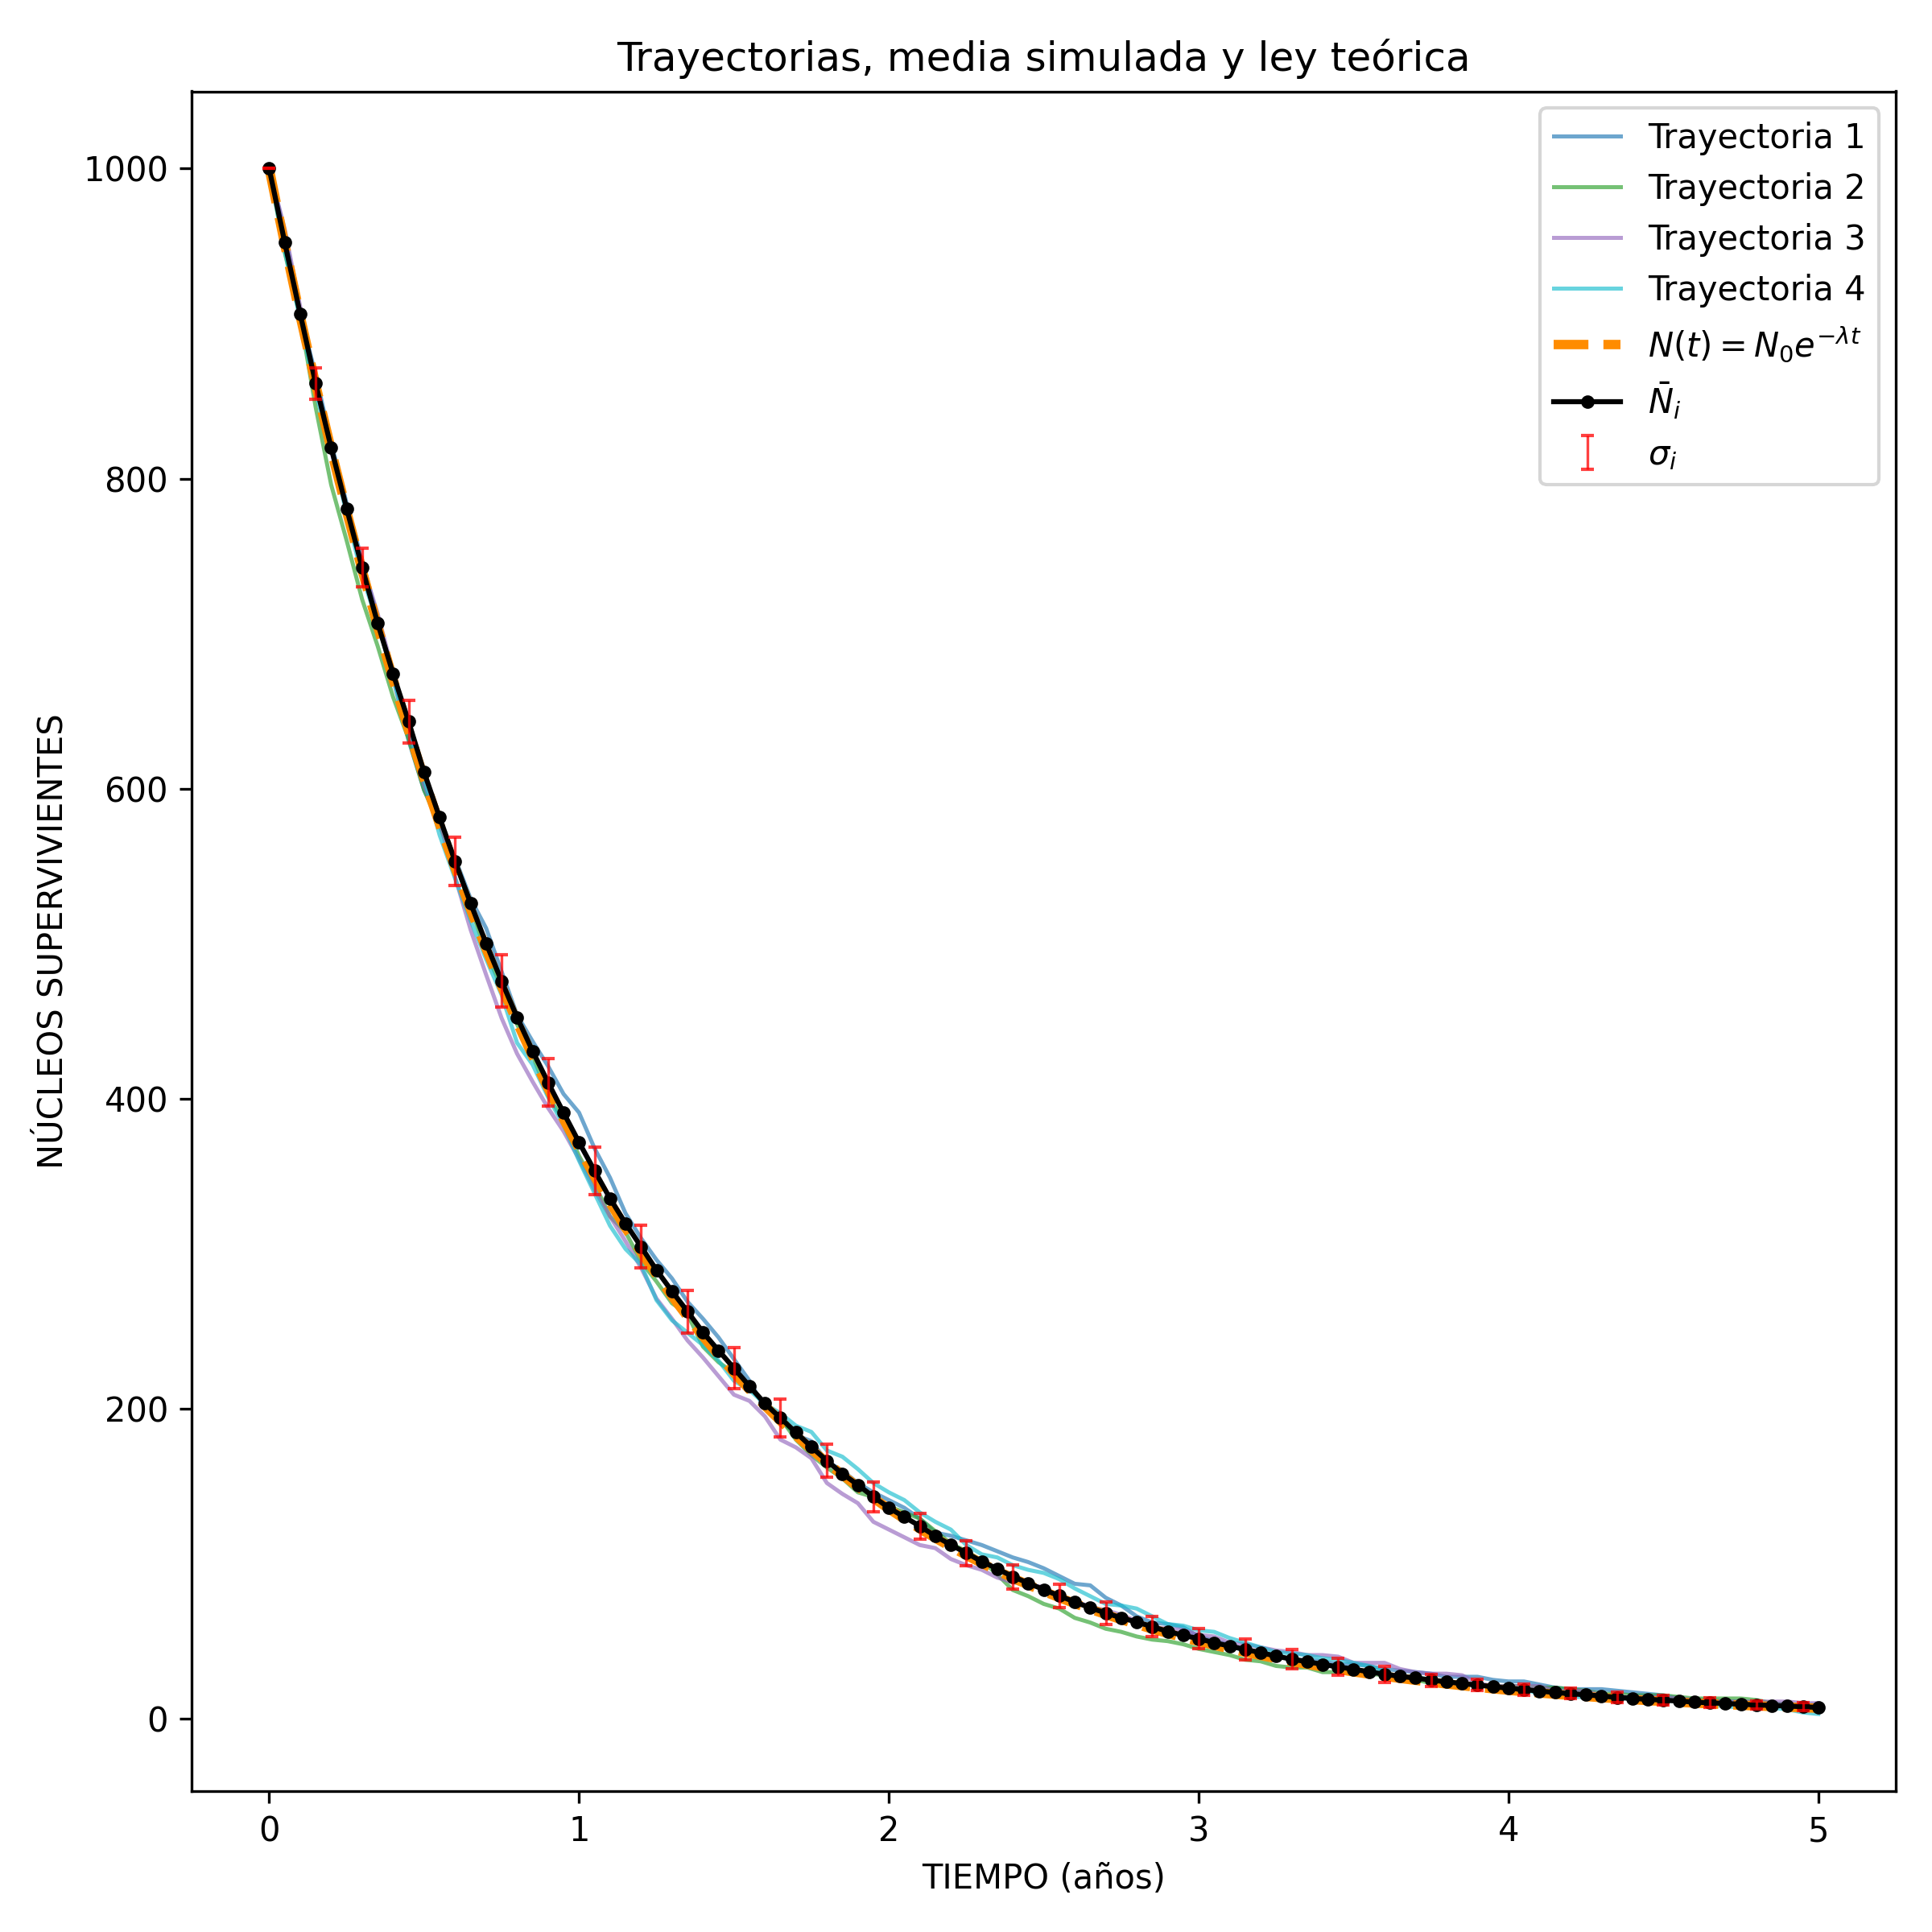
\includegraphics[width=1\textwidth]{TAREA4/figura1_trayectorias.png}
\caption{Cuatro trayectorias escogidas aleatoriamente entre un total de 50 simulaciones, comparadas con el valor medio y la desviación típica del número de núcleos supervivientes en cada intervalo temporal.}
\label{fig:trayectorias_binomial}
\end{figure}

En la Figura~\ref{fig:trayectorias_binomial} se observa que las trayectorias individuales presentan fluctuaciones alrededor de la ley exponencial teórica. Estas fluctuaciones son consecuencia directa de la naturaleza aleatoria del proceso de desintegración. Sin embargo, al considerar el promedio de las 50 simulaciones, el resultado se aproxima de forma clara al comportamiento macroscópico esperado. Por tanto, aunque una trayectoria individual no reproduce exactamente la ley exponencial, el promedio estadístico del modelo binomial sí converge hacia ella.

\subsubsection{Convergencia con el número de simulaciones}

Una vez comprobado que el promedio de varias simulaciones reproduce la ley exponencial, se estudia cómo mejora esta aproximación al aumentar el número de las mismas. Para ello, se calcula la discrepancia relativa entre el valor medio simulado y el valor teórico en el tiempo de semivida ($t=T_{1/2}$).

En este instante, la ley de desintegración radiactiva predice

$$
N(T_{1/2})=\frac{N_0}{2}.
$$

Por tanto, se define el error relativo como

$$
\Delta(T_{1/2})=
\frac{
\left|\overline{N}(T_{1/2})-N(T_{1/2})\right|
}{
N(T_{1/2})
}.
$$

\begin{figure}[H]
\centering
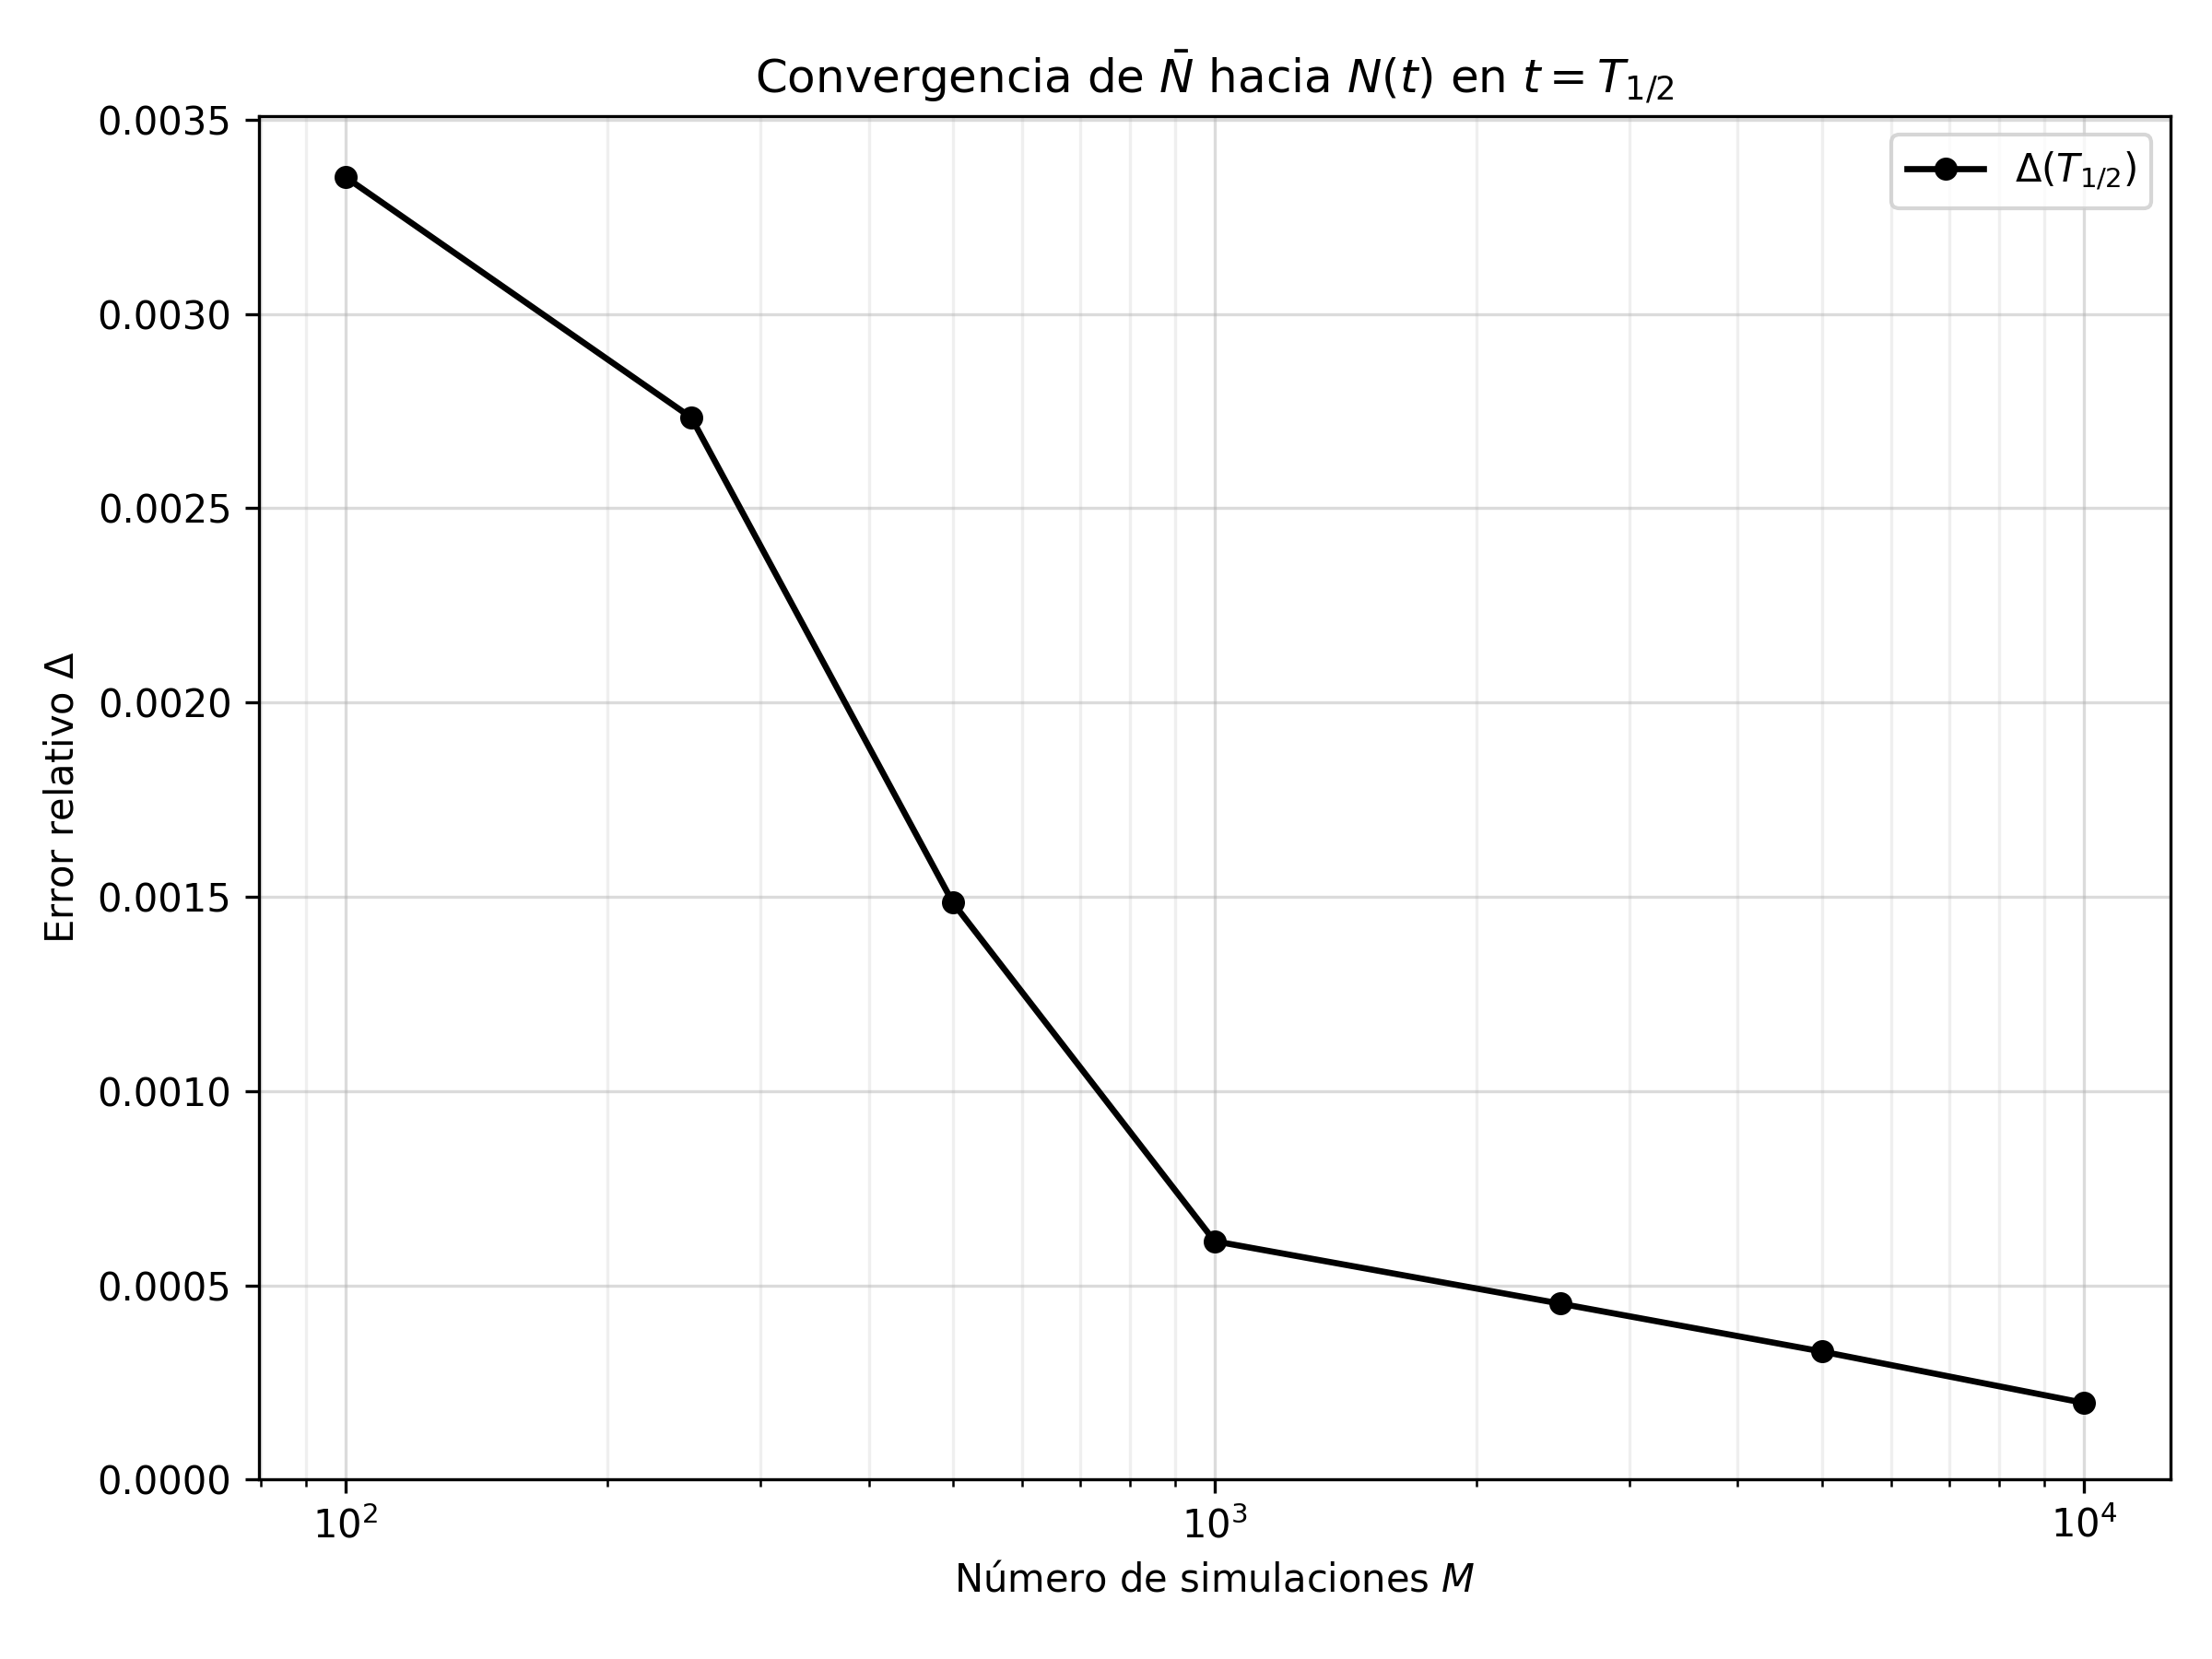
\includegraphics[width=1\textwidth]{TAREA4/figura2_convergencia_t12.png}
\caption{Error relativo entre el valor medio simulado y el valor teórico en el tiempo de semivida $T_{1/2}$, en función del número de simulaciones (M).}
\label{fig:convergencia_semivida}
\end{figure}

En la Figura~\ref{fig:convergencia_semivida} se observa que la discrepancia relativa disminuye al aumentar el número de simulaciones. Esto indica que el promedio estadístico obtenido mediante el modelo binomial converge hacia el valor predicho por la ley macroscópica de desintegración radiactiva.

\begin{cajadefinicion}
  La reducción de esta discrepancia al aumentar $M$ está relacionada con el comportamiento estadístico de la media muestral. Si se considera un instante fijo $t_i$, cada simulación proporciona un valor $N_i^{(j)}$. Al tratarse de realizaciones independientes, si la varianza asociada a una trayectoria individual es $\sigma_i^2$, la varianza del valor medio viene dada por

\begin{equation}
\mathrm{Var}(\overline{N}_i)
=
\mathrm{Var}\left(
\frac{1}{M}\sum_{j=1}^{M}N_i^{(j)}
\right).
\end{equation}

Como las simulaciones son independientes, la varianza de la suma es la suma de las varianzas. Por tanto,

\begin{equation}
\mathrm{Var}(\overline{N}_i)
=
\frac{1}{M^2}
\sum_{j=1}^{M}
\mathrm{Var}\left(N_i^{(j)}\right)
=
\frac{1}{M^2}M\sigma_i^2
=
\frac{\sigma_i^2}{M}.
\end{equation}

La desviación típica asociada al valor medio será entonces

\begin{equation}
\sigma_{\overline{N}_i}
=
\sqrt{\mathrm{Var}(\overline{N}_i)}
=
\frac{\sigma_i}{\sqrt{M}}.
\end{equation}

Esto indica que la incertidumbre estadística del promedio disminuye como $1/\sqrt{M}$. Por ello, al aumentar el número de simulaciones, se espera que el valor medio simulado se aproxime progresivamente al valor teórico, aunque el error relativo $\Delta$ no tenga por qué decrecer de forma perfectamente monótona para todos los valores de $M$.
\end{cajadefinicion}


\subsubsection{Error relativo máximo}

El análisis anterior permite estudiar la convergencia del modelo en un instante concreto, el tiempo de semivida. Sin embargo, para comprobar la precisión global de la simulación, también es necesario analizar la discrepancia entre el valor medio simulado y el valor teórico en todos los instantes temporales.

Para ello, se calcula el error relativo en cada instante $t_i$,

\begin{equation}
\Delta_i=
\frac{
\left|\overline{N}_i-N(t_i)\right|
}{
N(t_i)
},
\label{eq:error_relativo_ti}
\end{equation}

y posteriormente se toma el valor máximo de dicha discrepancia,

\begin{equation}
\Delta_{\max}=
\max(\Delta_i).
\label{eq:error_relativo_maximo}
\end{equation}

De esta forma, $\Delta_{\max}$ representa el mayor error relativo cometido por la simulación a lo largo de todo el intervalo temporal estudiado.

\begin{figure}[H]
\centering
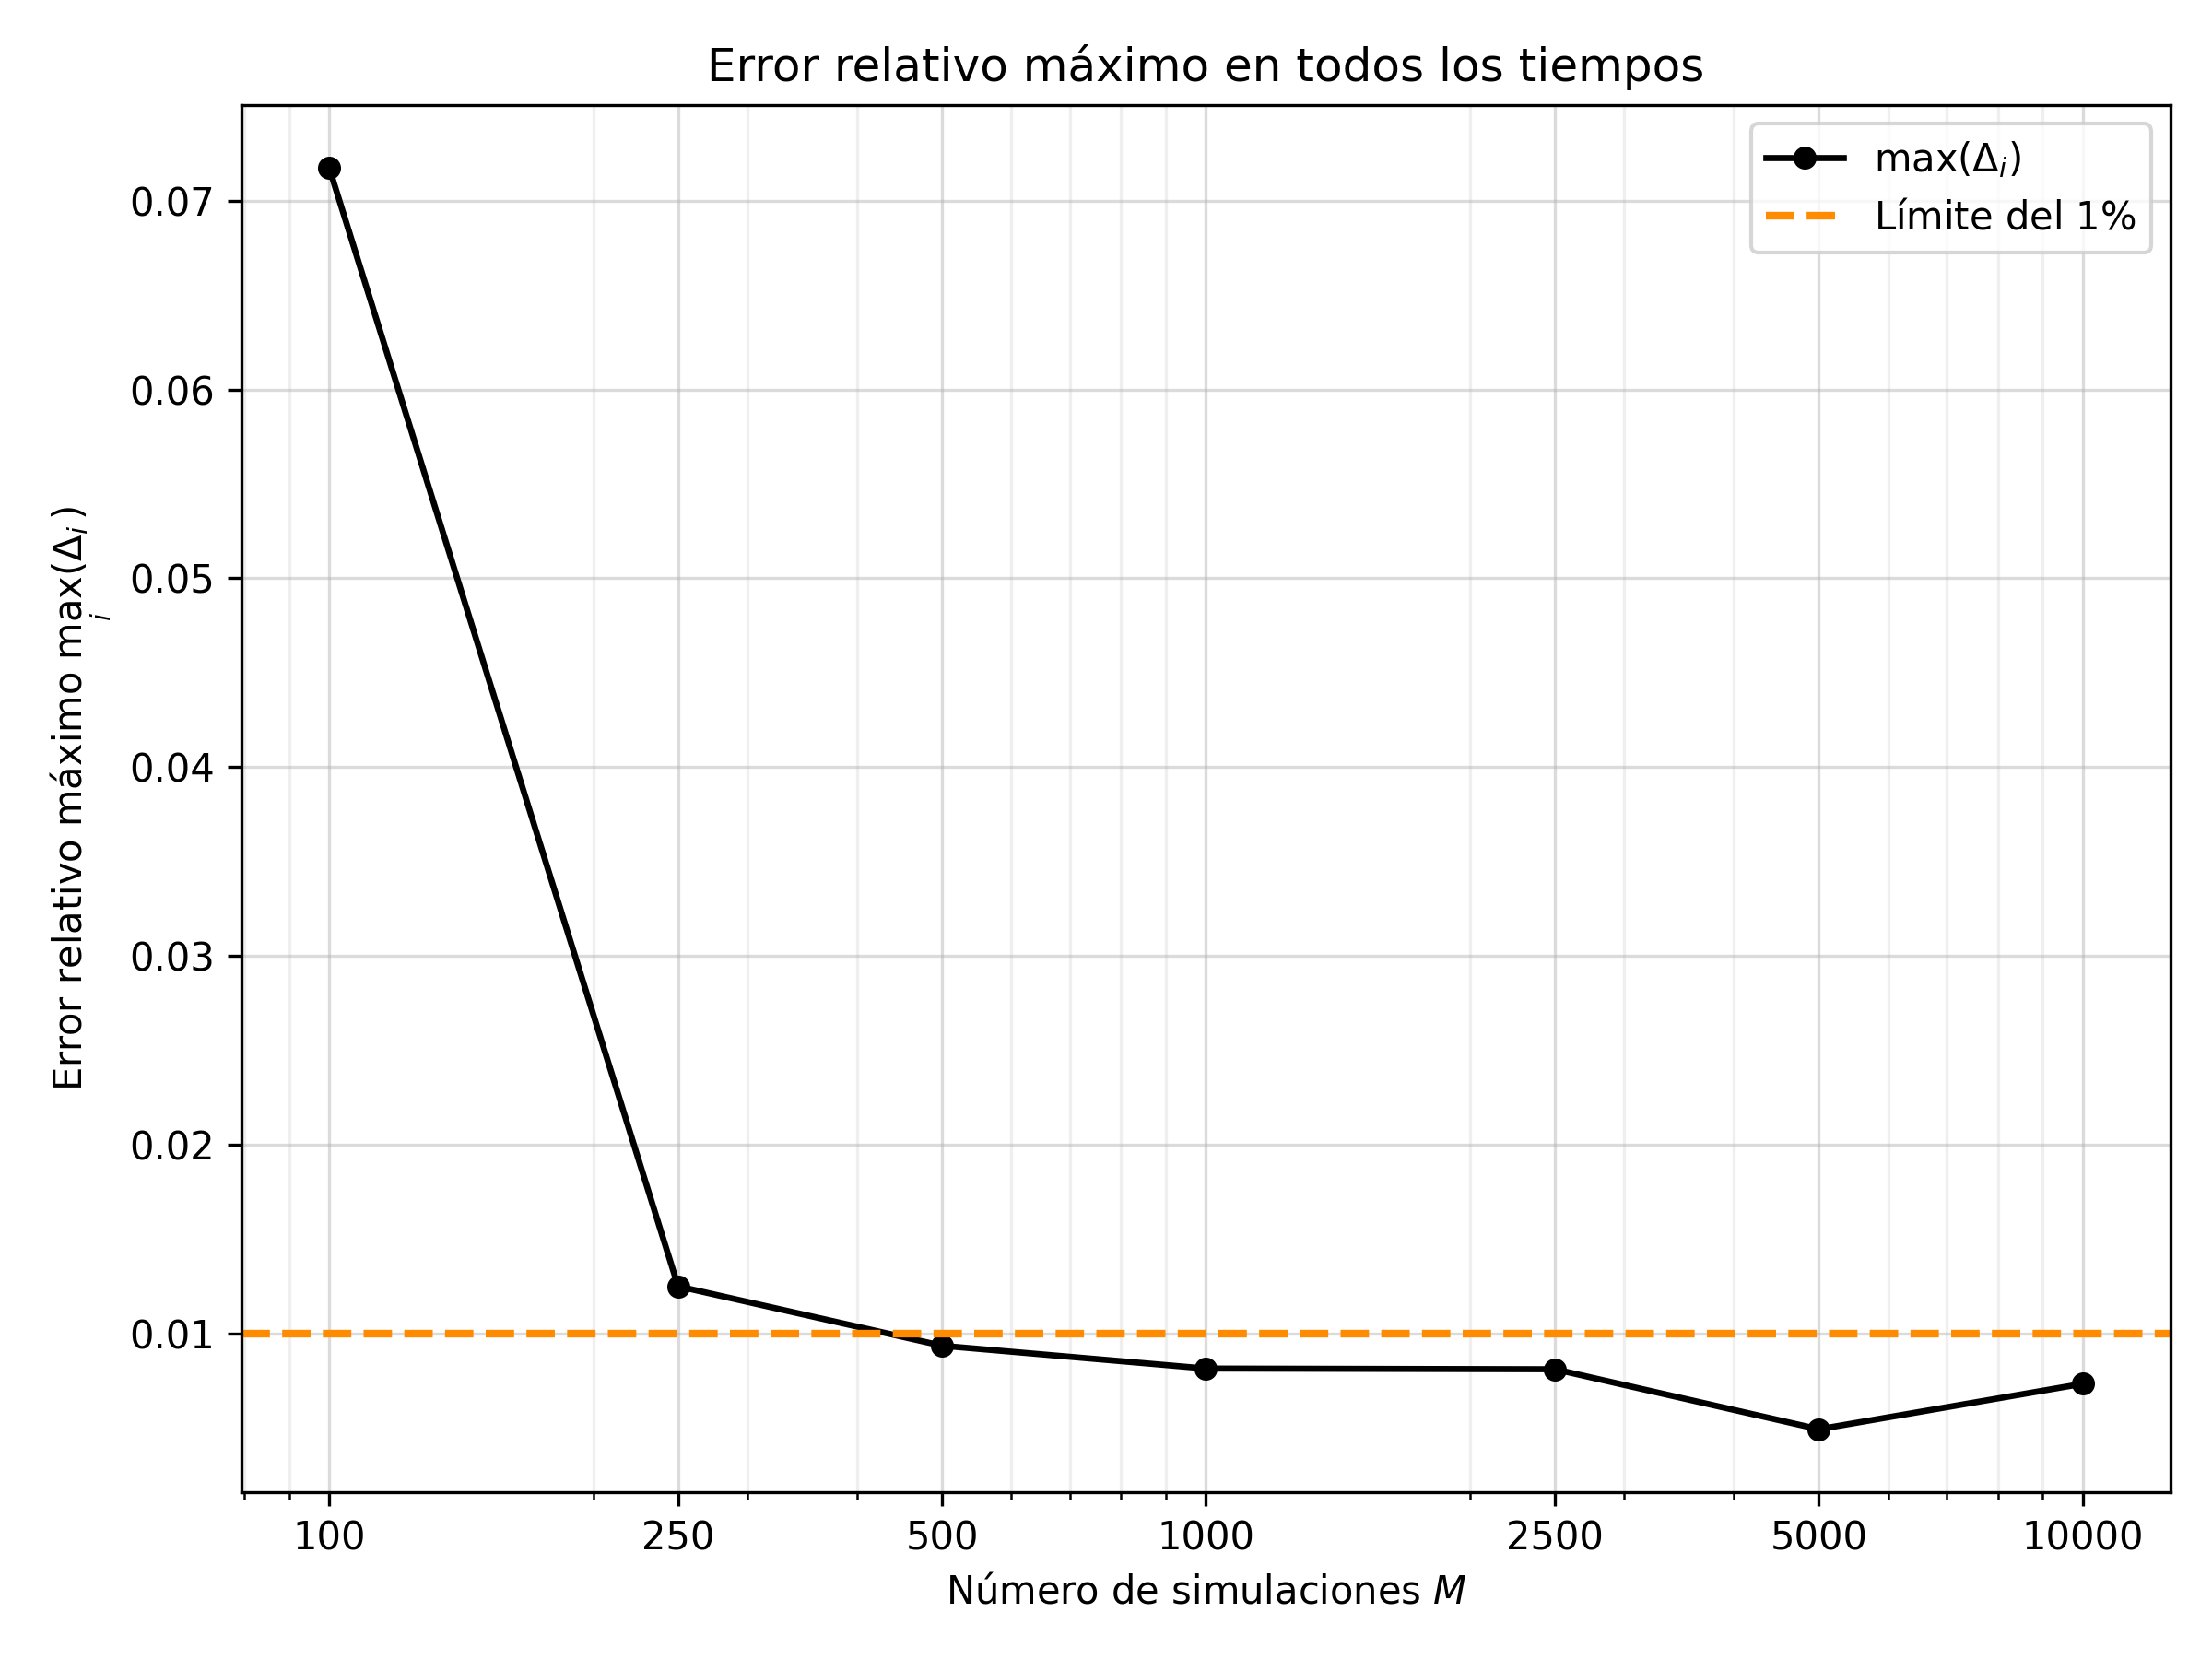
\includegraphics[width=1\textwidth]{TAREA4/error_maximo_vs_M.png}
\caption{Error relativo máximo entre el valor medio simulado y el valor teórico considerando todos los instantes temporales, en función del número de simulaciones (M). La línea discontinua indica el límite del $1\%$.}
\label{fig:error_relativo_maximo}
\end{figure}

En la Figura \ref{fig:error_relativo_maximo} se observa que el error relativo máximo disminuye de forma notable al aumentar el número de simulaciones. Para $M=100$, la discrepancia máxima es superior al $1\%$, lo que indica que el promedio obtenido todavía no reproduce con suficiente precisión la ley teórica en todos los instantes temporales. Sin embargo, a partir de $M=500$, el error relativo máximo queda por debajo del límite del $1\%$ en la realización mostrada.

Debido a la naturaleza aleatoria del método Monte Carlo, esta tendencia no tiene por qué reproducirse de forma idéntica en todas las ejecuciones. Al repetir el análisis pueden aparecer oscilaciones puntuales, incluso para valores de $M$ superiores a 500. No obstante, la tendencia general observada es estable: al aumentar $M$, el error relativo máximo tiende a reducirse, y el valor $M=500$ se sitúa en torno al umbral del $1\%$. Por ello, este valor puede tomarse como una estimación razonable del número mínimo de simulaciones necesario para obtener una precisión global del orden del $1\%$.


\subsection{Dependencia estadística con el número inicial de núcleos}

Antes de continuar con el análisis estadístico del modelo, se estudia la dependencia de las fluctuaciones con el número inicial de núcleos $N_0$. Este estudio permite cuantificar cómo varían la desviación típica absoluta y la desviación típica relativa al aumentar el tamaño del sistema simulado, proporcionando un criterio para escoger valores de $N_0$ adecuados.

Sea $t^*$ un valor de tiempo fijo, la desviación típica teórica (\ref{eq:desviación_típica_binomial}) es

\begin{equation}
\sigma_N=
\sqrt{
N_0e^{-\lambda t^*}\left(1-e^{-\lambda t^*}\right)
}.
\label{eq:desviacion_tipica_supervivientes_t_estrella}
\end{equation}

Como $t^*$ se mantiene fijo, los factores $e^{-\lambda t^*}$ y $1-e^{-\lambda t^*}$ son constantes. Por tanto, la dependencia de la desviación típica con el número inicial de núcleos es

\begin{equation}
\sigma_N \propto \sqrt{N_0}.
\label{eq:sigma_proporcional_raiz_N0}
\end{equation}

La desviación típica $\sigma_N$ mide la dispersión absoluta del número de núcleos supervivientes. Sin embargo, para saber si esta dispersión es grande o pequeña en comparación con el valor medio, se introduce la desviación típica relativa

\begin{equation}
\frac{\sigma_N}{\overline{N}} = 
\frac{
\sqrt{
N_0e^{-\lambda t^*}\left(1-e^{-\lambda t^*}\right)
}
}{
N_0e^{-\lambda t^*}
}.
\label{eq:desviacion_relativa_supervivientes}
\end{equation}

Simplificando,

\begin{equation}
\frac{\sigma_N}{\overline{N}}
 = \sqrt{
\frac{
1-e^{-\lambda t^*}
}{
N_0e^{-\lambda t^*}
}
}.
\label{eq:desviacion_relativa_simplificada}
\end{equation}

Como el instante $t^*$ es fijo, la dependencia con $N_0$ queda dada por

\begin{equation}
\frac{\sigma_N}{\overline{N}}
\propto
\frac{1}{\sqrt{N_0}}.
\label{eq:desviacion_relativa_proporcional_raiz_N0}
\end{equation}


Por tanto, al aumentar el número inicial de núcleos, la desviación típica absoluta aumenta como $\sqrt{N_0}$, pero la desviación típica relativa disminuye como $1/\sqrt{N_0}$. Esto significa que, aunque las fluctuaciones absolutas sean mayores para sistemas con más núcleos, dichas fluctuaciones representan una fracción cada vez menor del valor medio.

Para comprobar numéricamente este comportamiento, se realiza la simulación en el instante $t^*=T_{1/2}$ para distintos valores de $N_0$. Para cada valor de $N_0$, se calcula el valor medio $\overline{N}$, la desviación típica $\sigma_N$ y la desviación típica relativa $\sigma_N/\overline{N}$.

\begin{figure}[H]
\centering
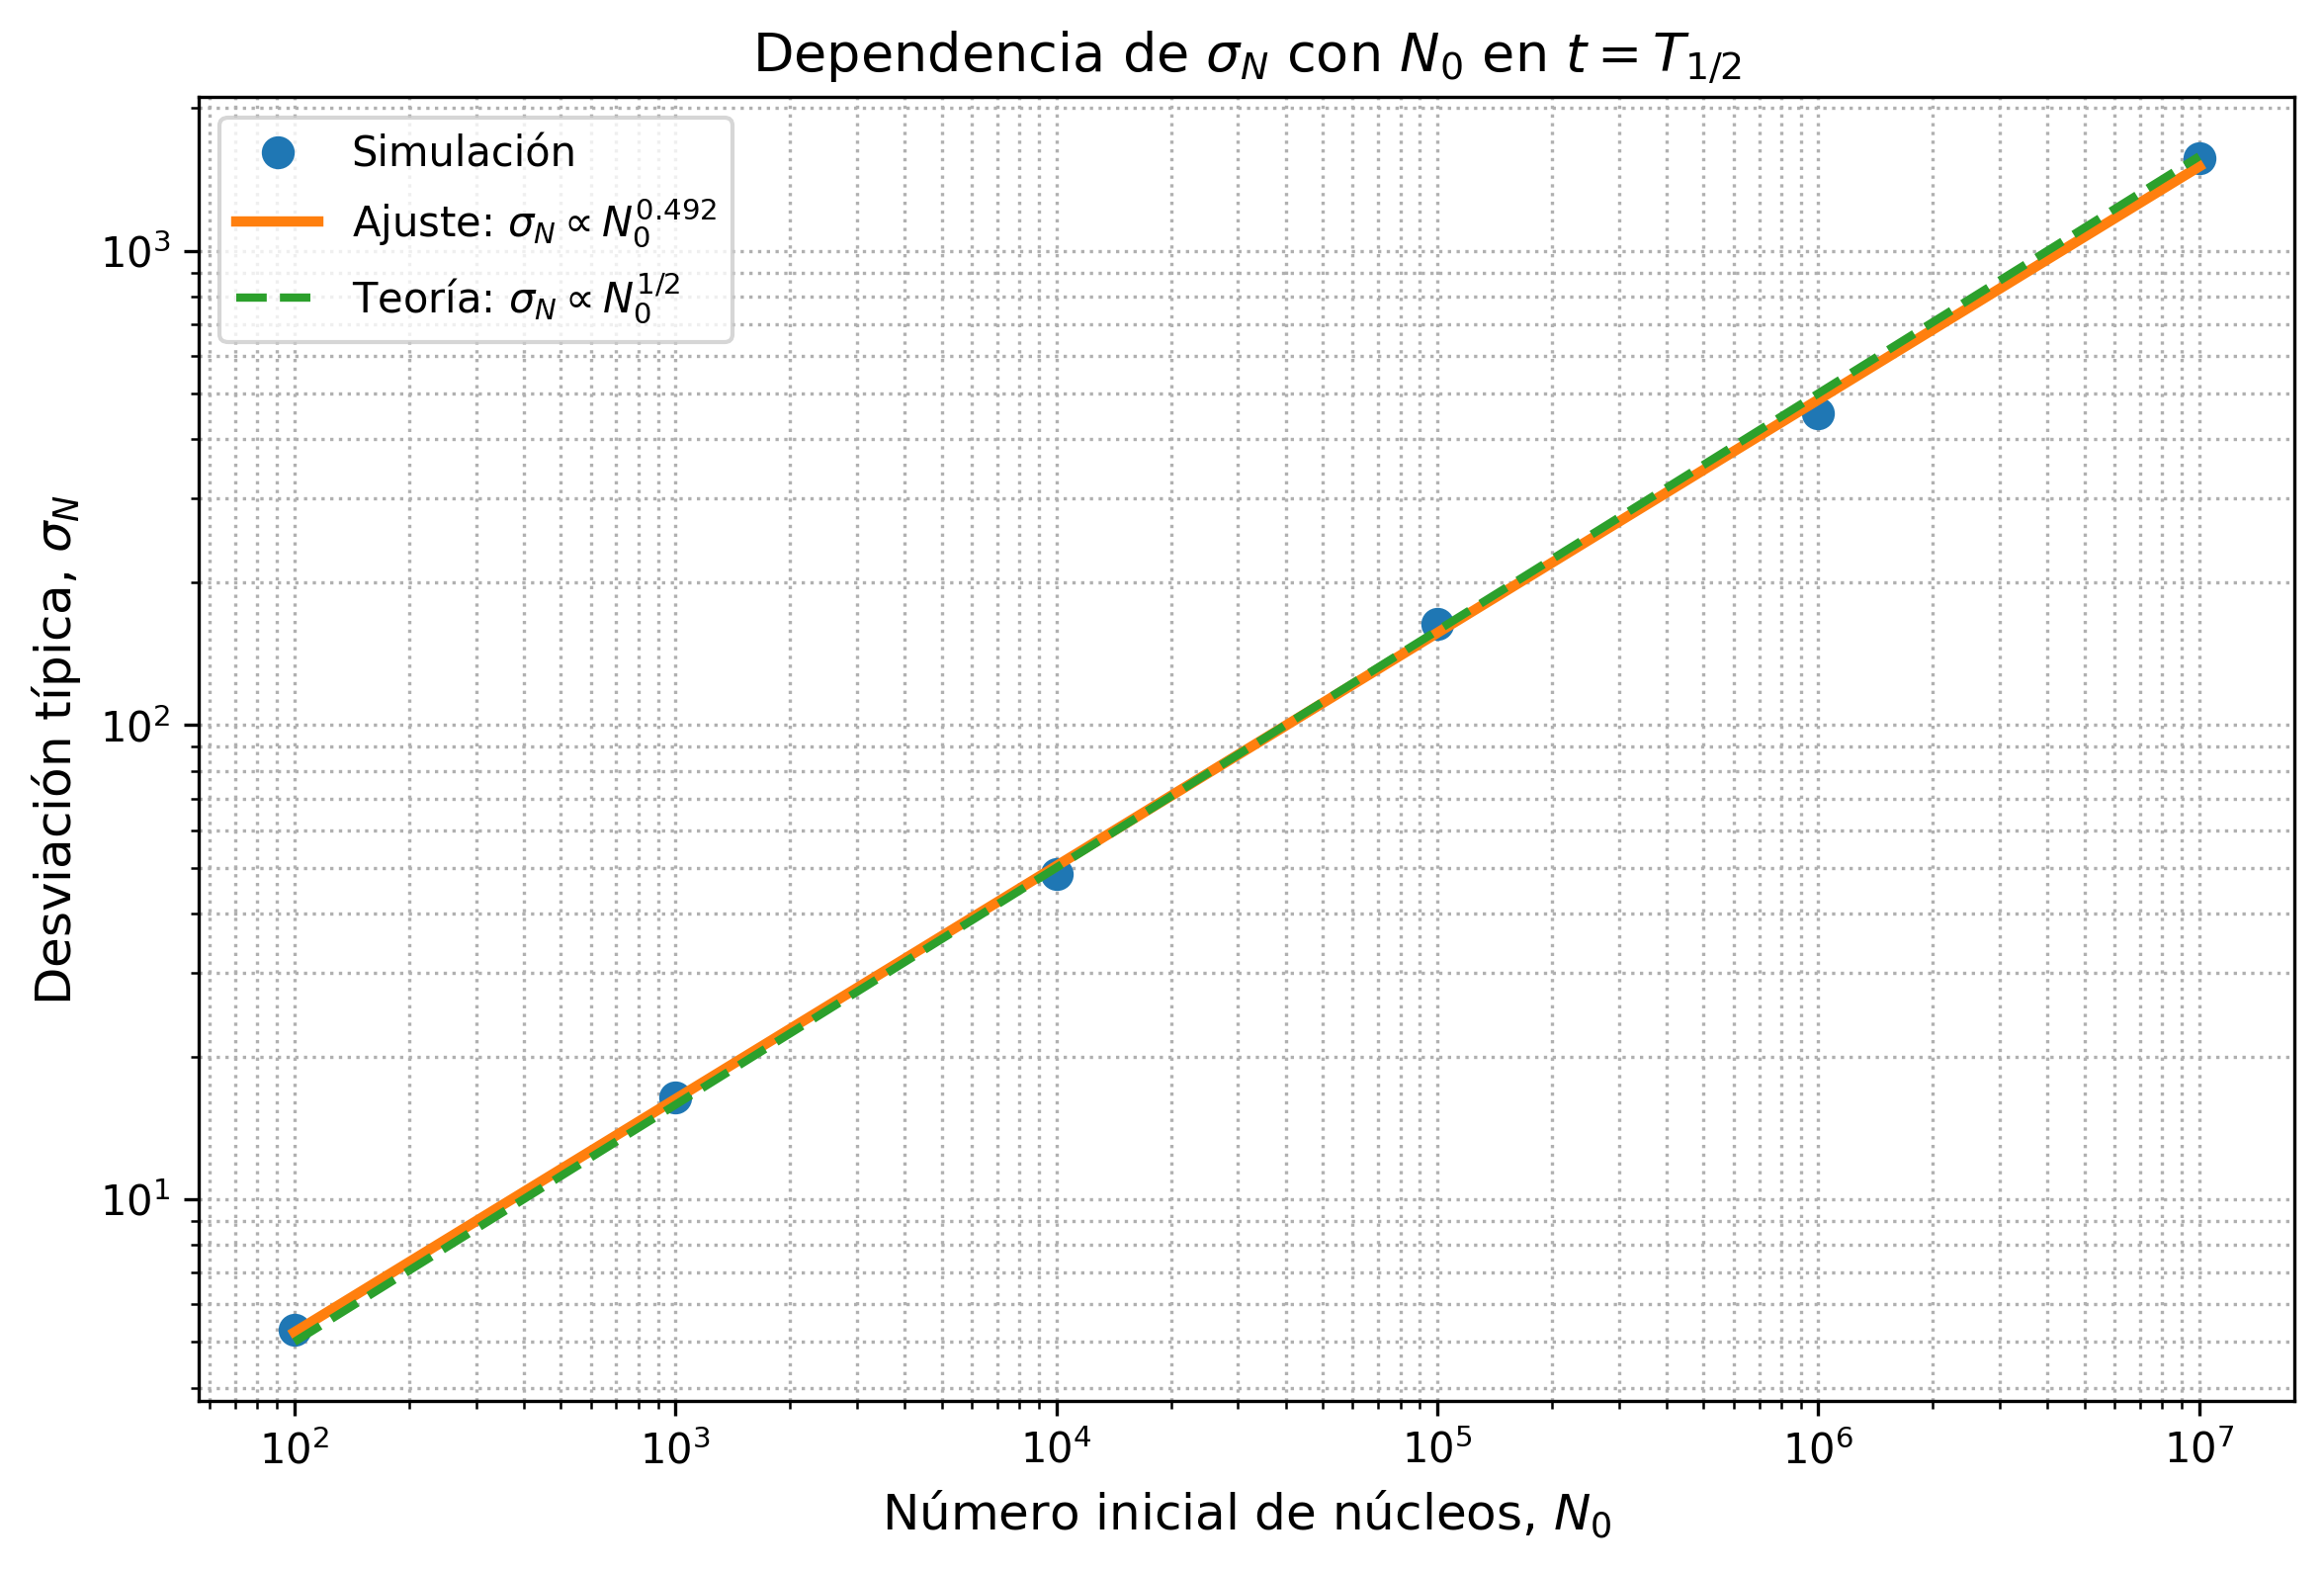
\includegraphics[width=1\textwidth]{TAREA6/desviacion_tipica_vs_N0.png}
\label{fig:desviacion_tipica_vs_N0}
\caption{Desviación típica frente a $N_0$.}
\end{figure}

\begin{figure}[H]
\centering
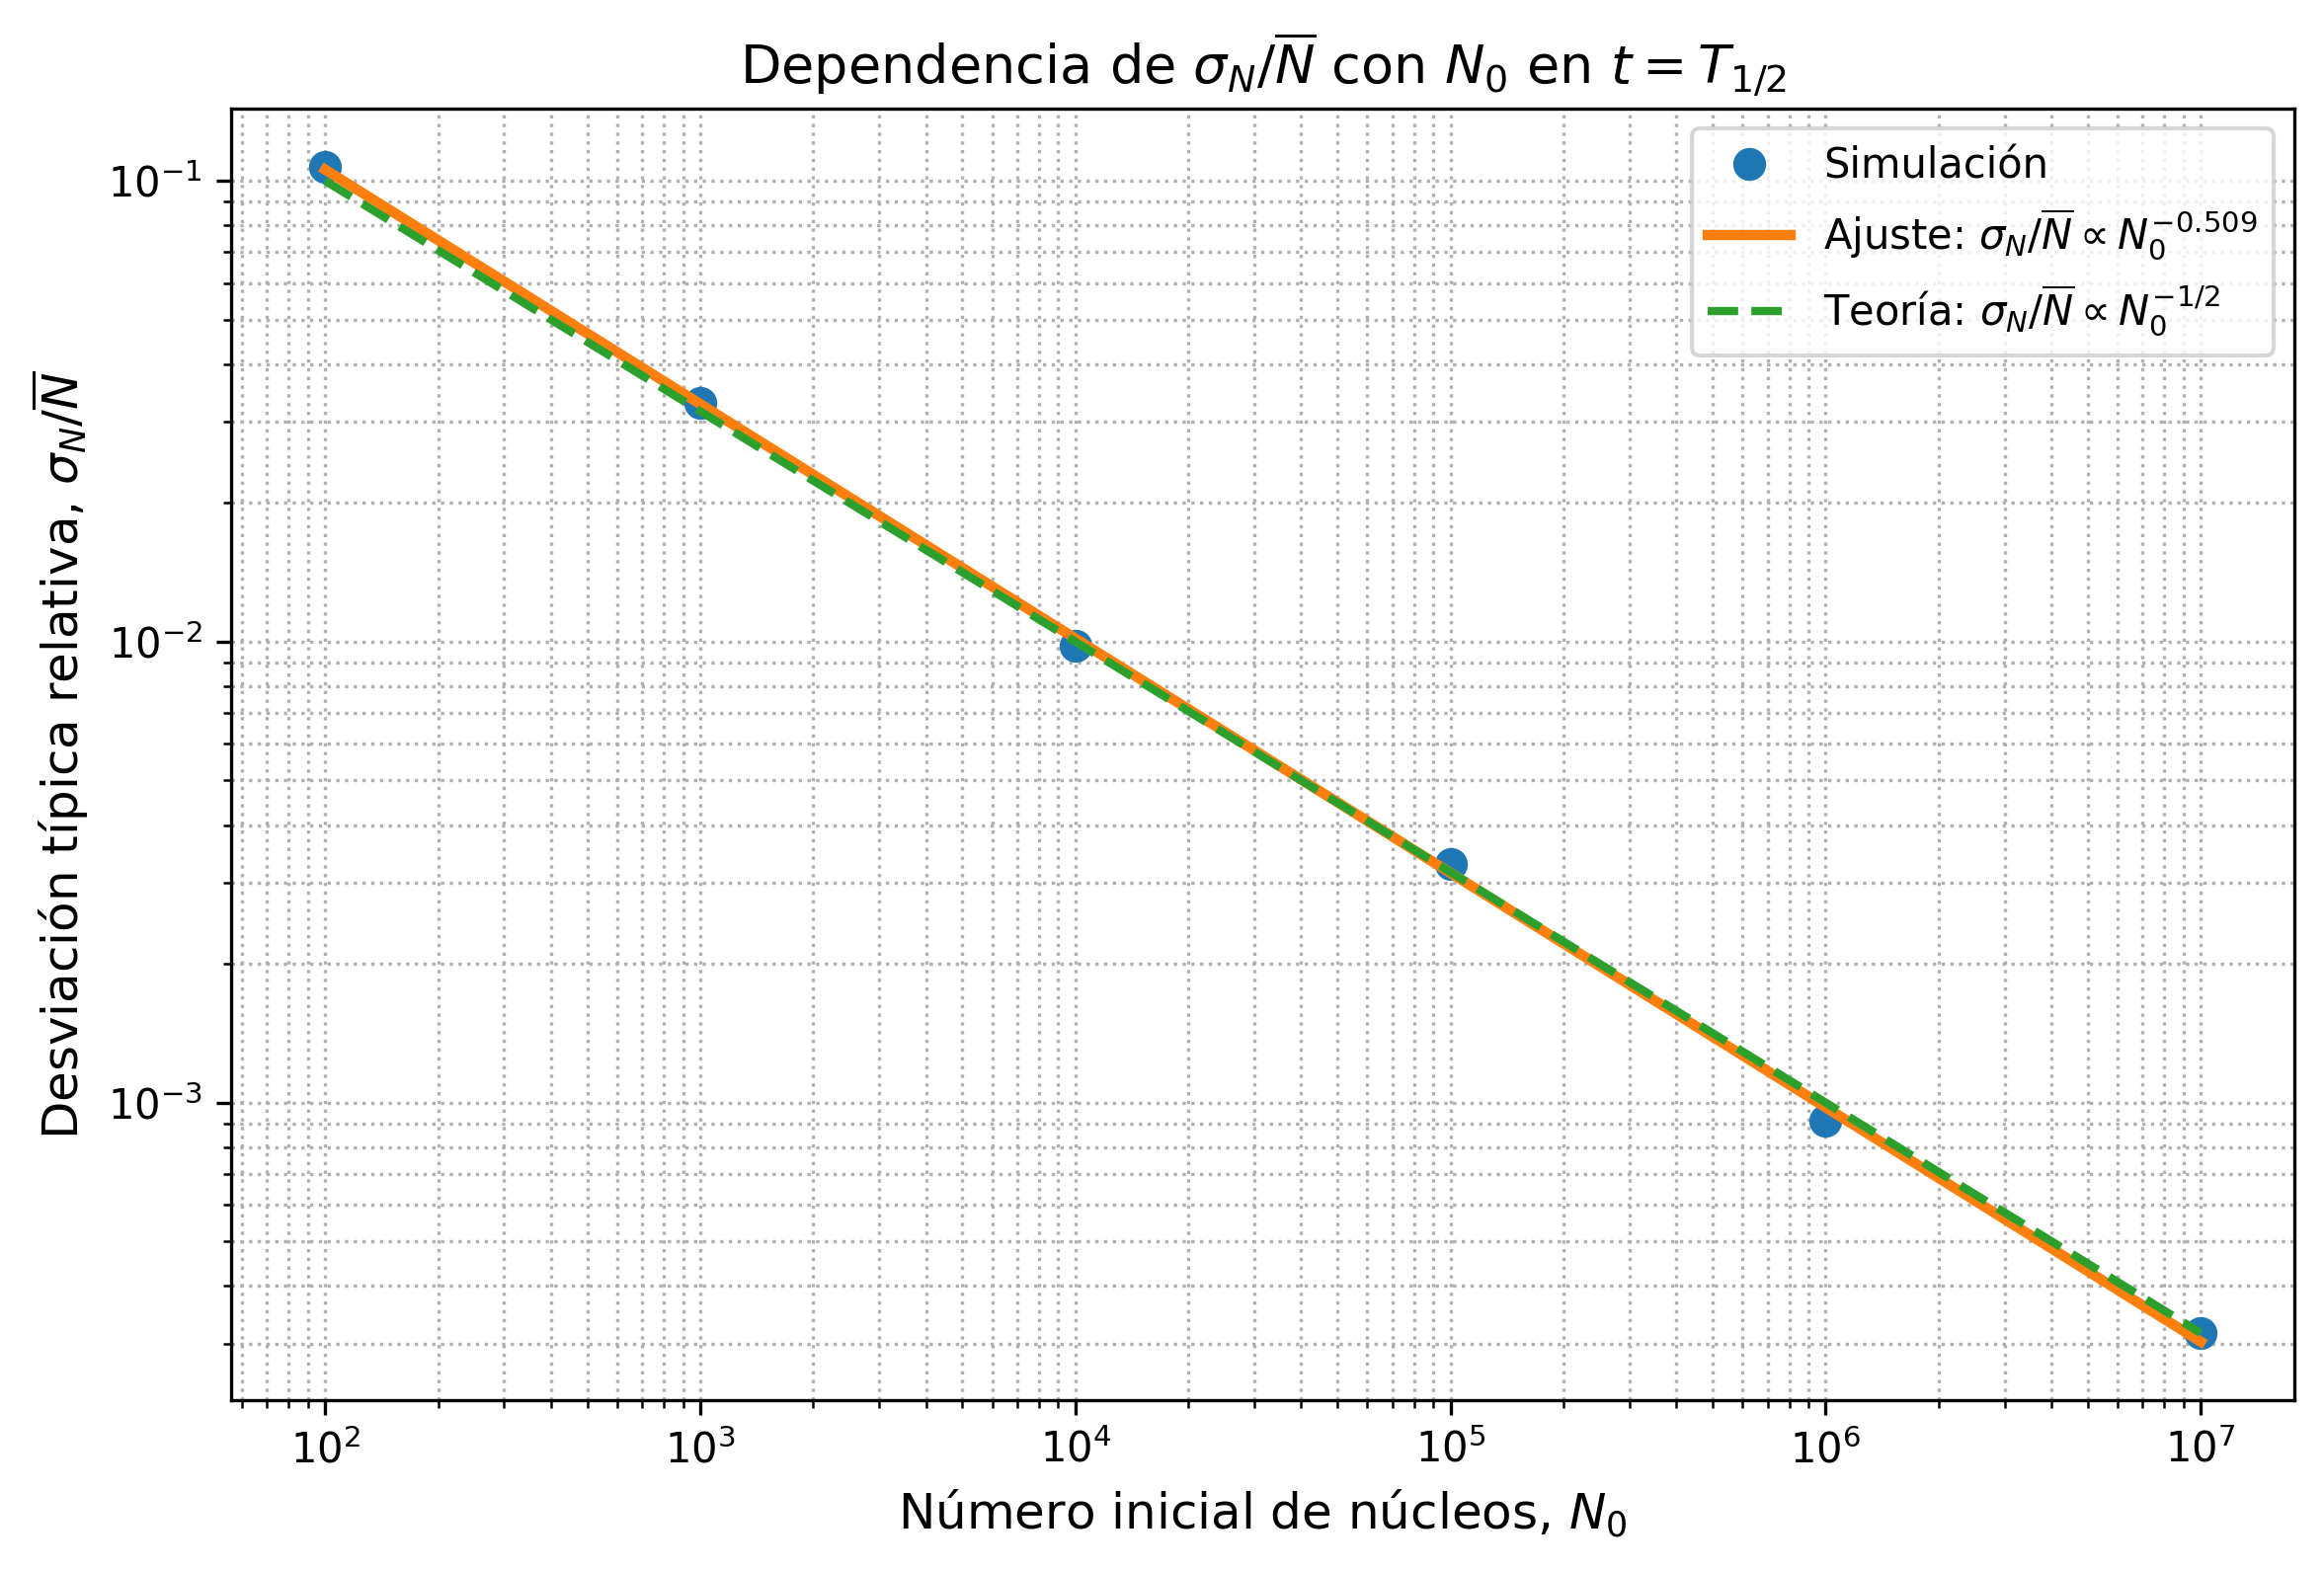
\includegraphics[width=1\textwidth]{TAREA6/desviacion_relativa_vs_N0.png}
\label{fig:desviacion_relativa_vs_N0}
\caption{Desviación típica relativa frente a $N_0$.}
\end{figure}



Las representaciones en escala doble logarítmica muestran un comportamiento lineal, lo que confirma que ambas magnitudes siguen aproximadamente una ley de potencia con $N_0$. El ajuste realizado para la desviación típica proporciona un exponente próximo a $1/2$, mientras que el ajuste correspondiente a la desviación típica relativa da un exponente próximo a $-1/2$, dando consistencia a las dependencias teóricas obtenidas anteriormente.

Además, el análisis permite cuantificar la reducción de las fluctuaciones relativas al aumentar $N_0$. En el caso particular $t=T_{1/2}$, la desviación típica relativa viene dada por

\begin{equation}
\frac{\sigma_N}{\overline{N}}=\frac{1}{\sqrt{N_0}}.
\end{equation}

Por tanto, para $N_0=10^3$ se obtiene

\begin{equation}
\frac{\sigma_N}{\overline{N}}
=\frac{1}{\sqrt{1000}}
\simeq 0.032,
\end{equation}

lo que equivale aproximadamente a un $3.2\%$. Para $N_0=5000$,

\begin{equation}
\frac{\sigma_N}{\overline{N}}
=\frac{1}{\sqrt{5000}}
\simeq 0.014,
\end{equation}

por lo que la desviación relativa se reduce aproximadamente al $1.4\%$. Si se toma $N_0=10^4$, se obtiene

\begin{equation}
\frac{\sigma_N}{\overline{N}}
=\frac{1}{\sqrt{10000}}
\simeq
0.01,
\end{equation}

es decir, una desviación relativa del $1\%$.

Aunque el valor $N_0=10^4$ proporciona una reducción ligeramente mayor de las fluctuaciones relativas, la mejora respecto a $N_0=5000$ es moderada, pasando aproximadamente del $1.4\%$ al $1\%$. Por ello, en los análisis posteriores se emplea $N_0=5000$, que reduce de forma apreciable la dispersión relativa respecto al caso $N_0=10^3$, manteniendo un coste computacional menor que el correspondiente a $N_0=10^4$ y sin modificar el procedimiento de simulación.

\subsection{Distribución estadística de núcleos supervivientes y desintegrados}

Hasta ahora se ha comprobado que el promedio de muchas simulaciones reproduce la ley exponencial de desintegración radiactiva. Sin embargo, al tratarse de un proceso estocástico\footnote{Proceso cuya evolución se describe mediante variables aleatorias y, por tanto, mediante probabilidades.}, también es necesario analizar cómo se distribuyen los valores obtenidos alrededor de dicho promedio.

Para ello, se realizan $M=500$ simulaciones independientes con $N_0=5000$ núcleos iniciales, manteniendo fijos los parámetros $\lambda$, $dt$ y el tiempo total de simulación. A partir de estas simulaciones se seleccionan tres instantes temporales representativos,

%%% POR QUÉ SON REPRESENTATIVOS

\begin{equation}
t_I=\frac{T_{1/2}}{20},
\qquad
t_{II}=T_{1/2},
\qquad
t_{III}=5T_{1/2}.
\label{eq:tiempos_histogramas}
\end{equation}

En cada uno de estos instantes se obtiene una muestra formada por los valores del número de núcleos supervivientes,

\begin{equation}
\left(N_i^{(1)},N_i^{(2)},\dots,N_i^{(M)}
\right)
\label{eq:muestra_supervivientes}
\end{equation}

donde $i=I,II,III$ indica el instante temporal considerado y el superíndice $j=1,\dots,M$ identifica cada simulación independiente. De forma análoga, se obtiene la muestra correspondiente al número de núcleos desintegrados,

\begin{equation}
D_i^{(j)}=N_0-N_i^{(j)}.
\label{eq:nucleos_desintegrados_histogramas}
\end{equation}

\begin{cajadefinicion}
El número de intervalos del histograma se determina mediante la regla de Scott, que fija la anchura de los bines como

\begin{equation}
h=3.5\cdot\sigma\cdot M^{-1/3} \refmargen{Scott \cite{scott1979histograms}}{}
\label{eq:regla_scott}
\end{equation}

donde $\sigma$ es la desviación típica de la muestra y $M$ el número de datos.
\end{cajadefinicion}

Sobre cada histograma se superponen la distribución binomial teórica y la aproximación de Poisson, lo que permite comparar visualmente los resultados simulados con las distribuciones esperadas. Asimismo, se incluye en cada caso la media teórica (\ref{eq:media_distribucion_binomial}) y la media muestral (\ref{eq:valor_medio_Msimulaciones}) calculada a partir de la simulación.



\subsubsection{Histogramas de núcleos supervivientes}

\begin{figure}[H]
  \centering
  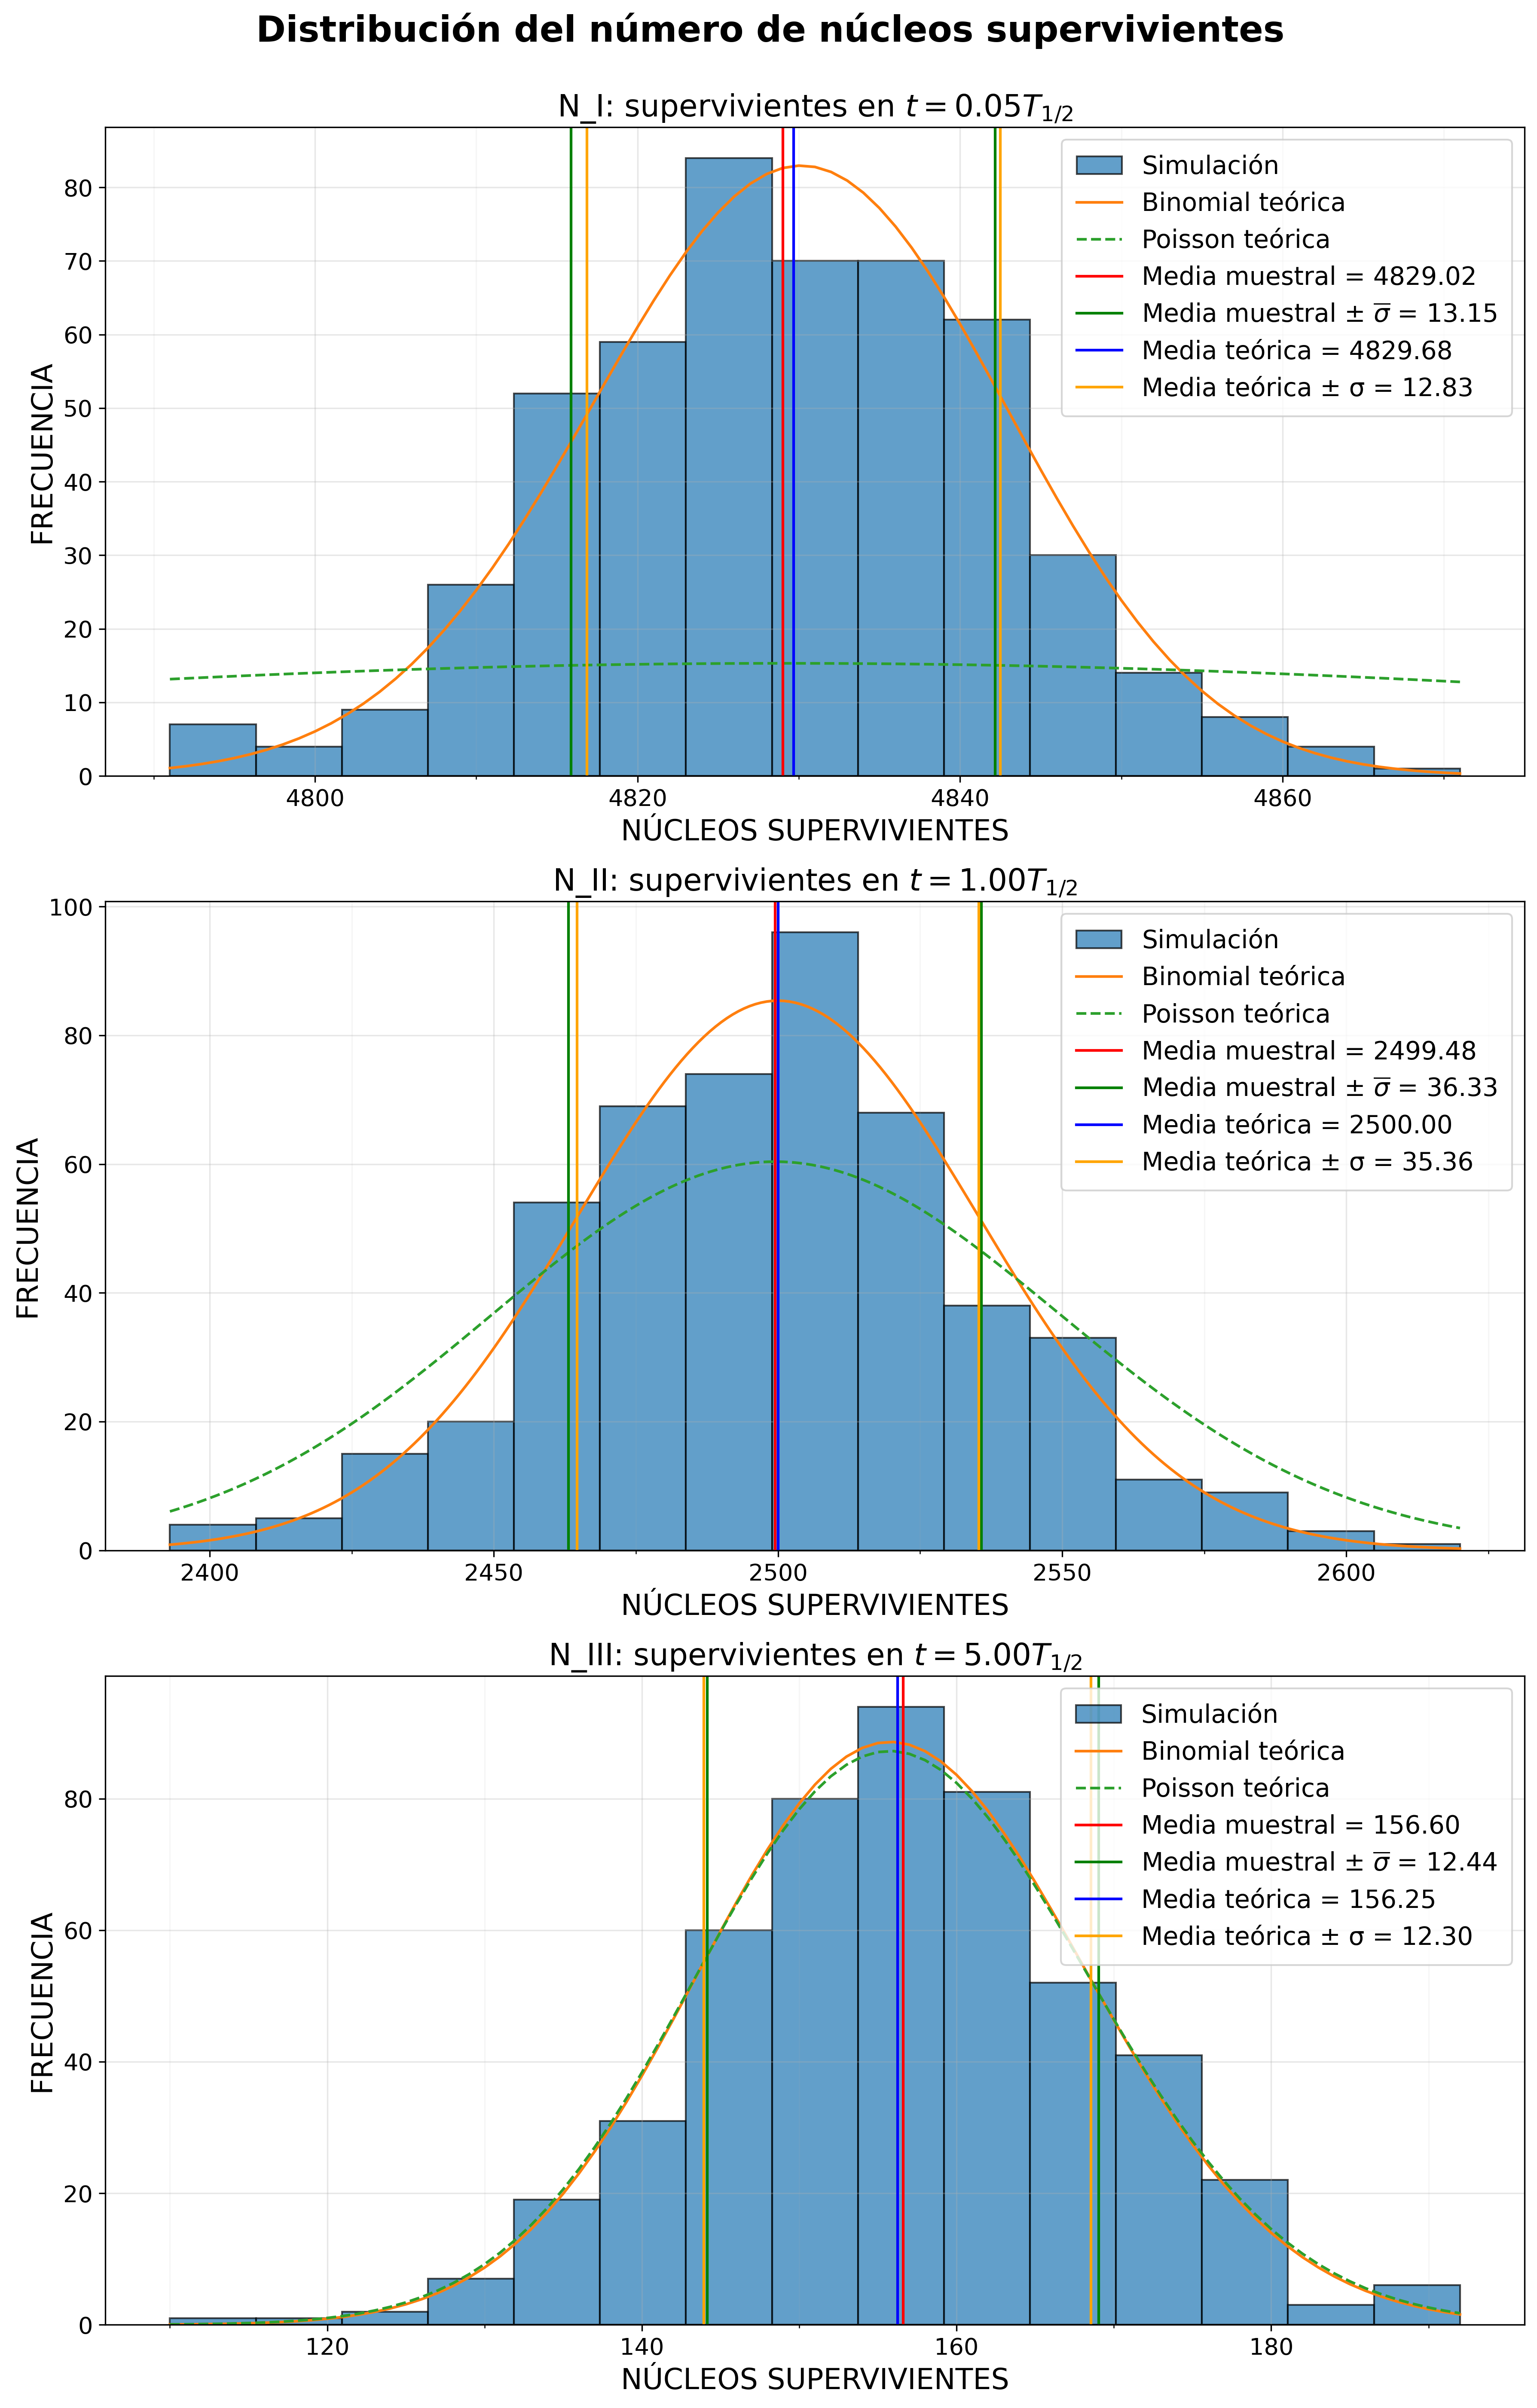
\includegraphics[width=1\textwidth]{TAREA5/histogramas_supervivientes_vertical.png}
  \label{fig:Histograma_supervivientes}
  \caption{Histogramas de núcleos supervivientes.}
\end{figure}

\subsubsection{Histogramas de núcleos desintegrados}

\begin{figure}[H]
  \centering
  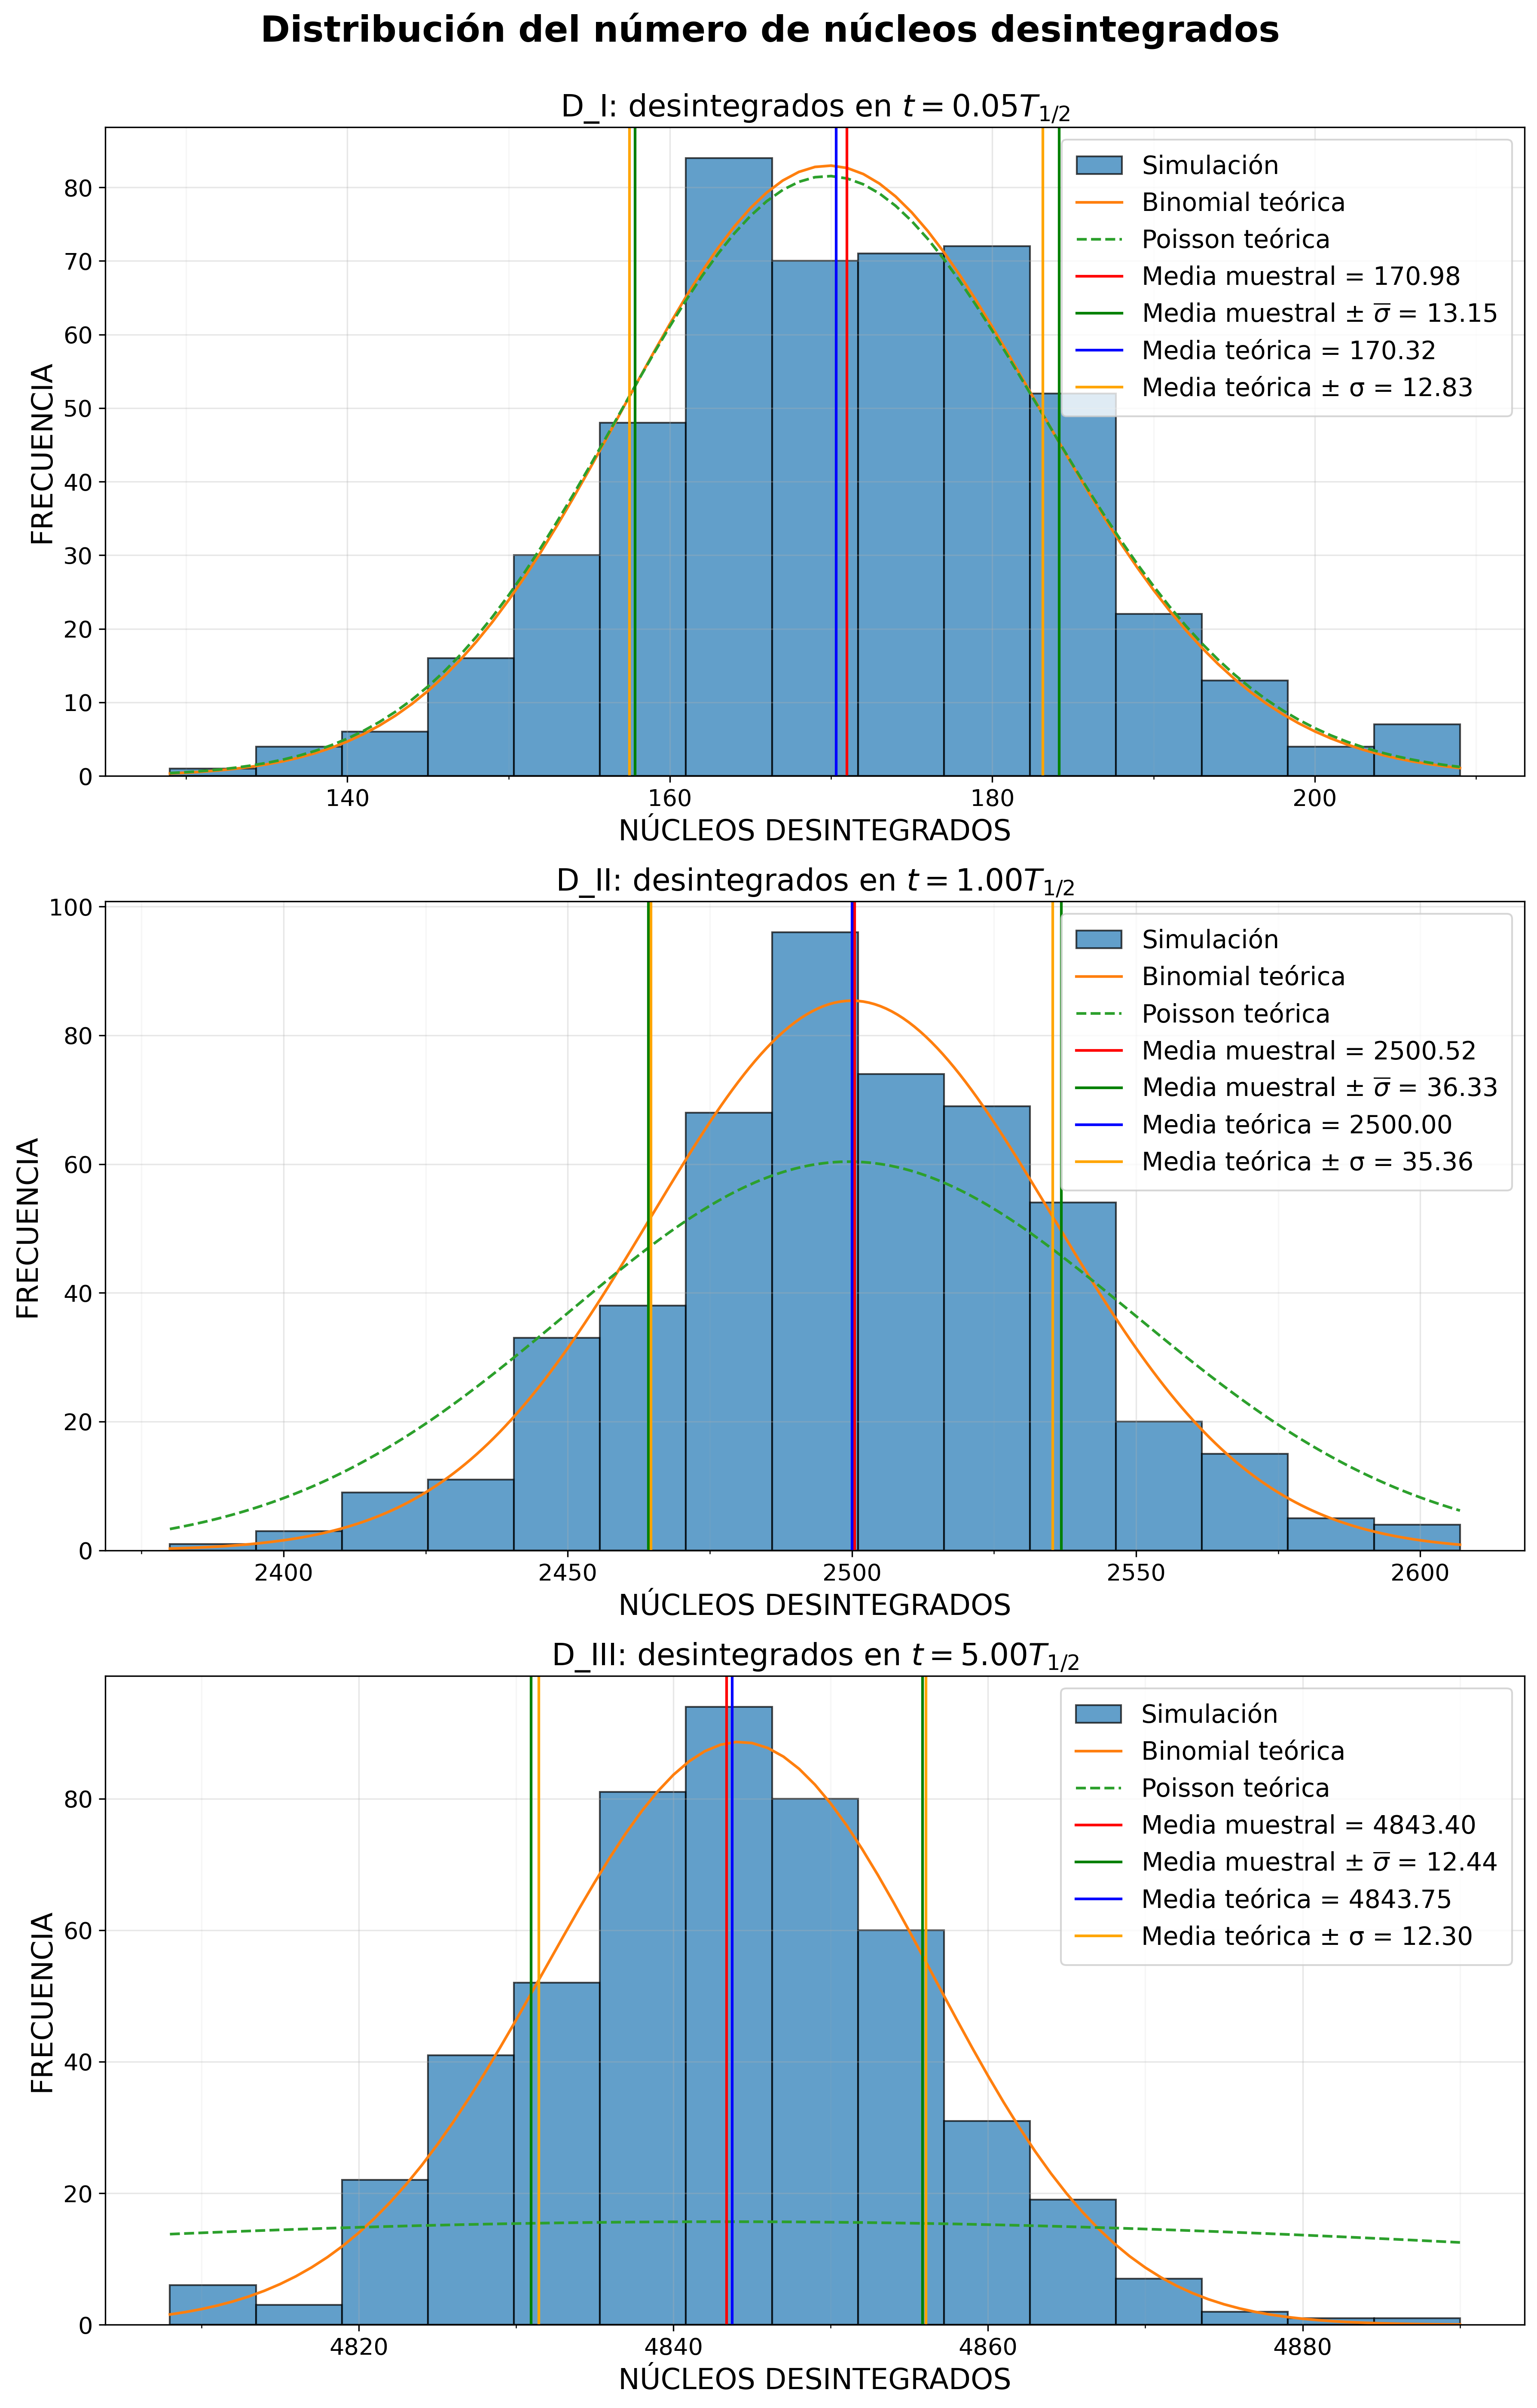
\includegraphics[width=1\textwidth]{TAREA5/histogramas_desintegrados_vertical.png}
  \label{fig:Histograma_desintegrados}
  \caption{Histogramas de núcleos desintegrados.}
\end{figure}

La distribución binomial reproduce adecuadamente las distribuciones de núcleos supervivientes y desintegrados. Esto se comprueba observando la proximidad entre las medias teóricas y muestrales, así como la forma de los histogramas.

La aproximación de Poisson, sin embargo, solo resulta adecuada cuando la probabilidad del suceso contado es pequeña. Por este motivo, describe correctamente el número de desintegraciones en tiempos cortos, como ocurre en $D_I$, y el número de supervivientes en tiempos avanzados, como ocurre en $N_{III}$.

Las distribuciones de núcleos supervivientes y desintegrados son complementarias, ya que el número de núcleos desintegrados queda determinado directamente por el número de supervivientes mediante la ecuación \ref{eq:nucleos_desintegrados_histogramas}.

Las líneas verticales asociadas a la media más y menos una desviación típica representan la dispersión característica de los valores obtenidos en las simulaciones. Por tanto, indican el intervalo en torno al valor medio en el que se concentra una parte significativa de la distribución. 

\subsubsection{Comparación cuantitativa entre las distribuciones binomial y de Poisson}

%%% CIFRAS SIGNIFICATIVAS

\begin{table}[H]
\centering
\resizebox{\textwidth}{!}{%
\begin{tabular}{c|cccccc}
\hline
Magnitud & $N_I$ & $N_{II}$ & $N_{III}$ & $D_I$ & $D_{II}$ & $D_{III}$ \\
\hline
$E(N)$ & 4829{,}682 & 2500{,}000 & 156{,}250 & 170{,}318 & 2500{,}000 & 4843{,}750 \\
$\sigma$ & 12{,}826 & 35{,}355 & 12{,}303 & 12{,}826 & 35{,}355 & 12{,}303 \\
$\overline{N}$ & 4829{,}014 & 2499{,}984 & 155{,}594 & 170{,}986 & 2500{,}016 & 4844{,}406 \\
$s$ & 13{,}006 & 35{,}623 & 12{,}346 & 13{,}006 & 35{,}623 & 12{,}346 \\
$\chi^2$ & 25{,}840 & 18{,}131 & 19{,}843 & 25{,}840 & 18{,}131 & 19{,}843 \\
$p$-value & 0{,}011 & 0{,}053 & 0{,}070 & 0{,}011 & 0{,}053 & 0{,}070 \\
\hline
\end{tabular}

}
\caption{Comparación entre las simulaciones Monte Carlo y la distribución binomial.}
\label{tab:comparacion_binomial}
\end{table}

\begin{table}[H]
\centering
\resizebox{\textwidth}{!}{%
\begin{tabular}{c|cccccc}
\hline
Magnitud & $N_I$ & $N_{II}$ & $N_{III}$ & $D_I$ & $D_{II}$ & $D_{III}$ \\
\hline
$E(N)$ & 4829{,}682 & 2500{,}000 & 156{,}250 & 170{,}318 & 2500{,}000 & 4843{,}750 \\
$\sigma$ & 69{,}50 & 50{,}00 & 12{,}50 & 13{,}05 & 50{,}00 & 69{,}60 \\
$\overline{N}$ & 4829{,}494 & 2497{,}242 & 156{,}890 & 170{,}506 & 2502{,}758 & 4843{,}110 \\
$s$ & 12{,}68 & 35{,}77 & 12{,}48 & 12{,}68 & 35{,}77 & 12{,}48 \\
$\chi^2$ & 357{,}463 & 63{,}721 & 18{,}117 & 12{,}848 & 64{,}260 & 253{,}759 \\
$p$-value & $<0{,}001$ & $<0{,}001$ & 0{,}079 & 0{,}460 & $<0{,}001$ & $<0{,}001$ \\
\hline
\end{tabular}

}
\caption{Comparación entre las simulaciones Monte Carlo y la aproximación de Poisson.}
\label{tab:comparacion_poisson}
\end{table}


Para la distribución binomial (\ref{tab:comparacion_binomial}), los valores teóricos de la esperanza $E(X)$ y de la desviación típica $\sigma$ son próximos a la media muestral $\overline{X}$ y a la desviación típica muestral $\overline{\sigma}$, respectivamente. Esto indica que la binomial reproduce correctamente tanto el valor central como la dispersión estadística de las simulaciones.

\begin{cajadefinicion}

Para cuantificar la calidad del ajuste, entre las distribuciones teóricas y los resultados simulados, se utiliza el estadístico $\chi^2$. Una vez fijados los intervalos del histograma, se compara la frecuencia observada $O_k$ en cada intervalo con la frecuencia esperada $E_k$ predicha por la distribución teórica considerada. El estadístico se calcula como \refmargen{NIST \cite{nist_chi_square}}{1.3.5.15}

\begin{equation}
\chi^2=\sum_{k=1}^{n_{\mathrm{bin}}}\frac{(O_k-E_k)^2}{E_k},
\end{equation}

donde $n_{\mathrm{bin}}$ es el número de intervalos empleados en el histograma.

Los grados de libertad se calculan como

\begin{equation}
\nu=n_{\mathrm{bin}}-1-r,
\end{equation}

donde $r$ representa el número de parámetros o restricciones adicionales asociadas a la distribución teórica. El término $-1$ aparece porque las frecuencias de los intervalos no son completamente independientes; al estar fijado el número total de simulaciones $M$, la frecuencia del último intervalo queda determinada por las anteriores. Por tanto, de los $n_{\mathrm{bin}}$ intervalos solo $n_{\mathrm{bin}}-1$ aportan información independiente.
\end{cajadefinicion}

En particular, se toma $r=2$ para la distribución binomial y $r=1$ para la aproximación de Poisson.

Con el valor de $\chi^2$ y los grados de libertad $\nu$ se obtiene el $p$-value, que mide hasta qué punto las diferencias observadas entre la distribución teórica y la simulación pueden atribuirse a fluctuaciones estadísticas. Se adopta como criterio un nivel de significación $\alpha=0.05$,\refmargen{NIST \cite{nist_pvalue}}{7.1.3.1} de forma que el ajuste se considera compatible con los datos cuando $p>0.05$.

De acuerdo con este criterio, los valores del $p$-value de la distribución binomial son superiores a $0.05$. Por tanto, no existen evidencias suficientes para rechazar el ajuste binomial en ninguno de los casos estudiados.

En cambio, la aproximación de Poisson muestra una validez más limitada. Esta aproximación solo supera el criterio en $D_I$ y en $N_{III}$, que corresponden a los casos en los que la probabilidad del suceso contado es pequeña. En $D_I$, el número de núcleos desintegrados es pequeño porque se considera un tiempo corto; en $N_{III}$, el número de núcleos supervivientes es pequeño porque se considera un tiempo avanzado.


\subsection{Estimación del tiempo de desintegración y propagación de incertidumbres}

En los apartados anteriores se ha seleccionado el modelo binomial como modelo de simulación y se ha comprobado que, al promediar un número suficiente de simulaciones independientes, reproduce el comportamiento macroscópico descrito por la ley exponencial de desintegración (\ref{eq:ley_desintegracion}). Además, el análisis de los histogramas ha mostrado que, en un instante temporal fijo, la distribución de núcleos supervivientes se describe adecuadamente mediante una distribución binomial. 

A partir de estos resultados, se puede estudiar cómo las fluctuaciones estadísticas del número de núcleos supervivientes se propagan a la estimación del tiempo transcurrido.

Partiendo de la ley macroscópica de desintegración (\ref{eq:ley_desintegracion}) se obtiene la ecuación (\ref{eq:tiempo_estimado}):

$$
t_{\mathrm{est}}=
-\frac{1}{\lambda}
\ln\left(\frac{N}{N_0}\right).
$$

Esta expresión permite interpretar cada resultado de la simulación como una estimación de la edad de la muestra. En particular, si $N$ representa el número de núcleos supervivientes obtenido en una simulación concreta, entonces $t_{\mathrm{est}}$ es el tiempo que se deduciría aplicando directamente la ley exponencial determinista(\ref{eq:ley_desintegracion}).


Sin embargo, debido a la naturaleza estocástica del proceso de desintegración, el número de núcleos supervivientes no toma siempre el mismo valor, sino que presenta fluctuaciones alrededor de su valor medio. Por tanto, la edad estimada mediante la ecuación (\ref{eq:tiempo_estimado}) también presenta una incertidumbre estadística.

\subsubsection{Propagación de errores estadísticos}

A partir de la ecuación (\ref{eq:tiempo_estimado}), considerando $N_0$ y $\lambda$ como constantes conocidas, se tiene

\begin{equation}
\sigma_t =
\left|
\frac{\partial t_{\mathrm{est}}}{\partial N}
\right|
\sigma_N.
\end{equation}

Como

\begin{equation}
\frac{\partial t_{\mathrm{est}}}{\partial N}
=
-\frac{1}{\lambda N},
\end{equation}

resulta

\begin{equation}
\sigma_t =
\frac{\sigma_N}{\lambda N}.
\label{eq:sigma_t_general}
\end{equation}

La desviación típica de la distribución binomial (\ref{eq:desviación_típica_binomial}) obtenida en la sección de la sección 3.2.3

$$
\sigma_N=\sqrt{N_0p(1-p)}.
$$

Sustituyendo esta expresión en la ecuación (\ref{eq:sigma_t_general}) y tomando $N=N_0p$, se obtiene

\begin{equation}
\sigma_t=
\frac{\sqrt{N_0p(1-p)}}{\lambda N_0p}.
\end{equation}

Por tanto,

\begin{equation}
\sigma_t=
\frac{1}{\lambda}
\sqrt{
\frac{1-p}{N_0p}
}.
\end{equation}

Finalmente, usando \(p=e^{-\lambda t}\), queda

\begin{equation}
\sigma_t=
\frac{1}{\lambda}
\sqrt{
\frac{e^{\lambda t}-1}{N_0}
}.
\label{eq:sigma_t_propagacion}
\end{equation}

Esta expresión muestra que la incertidumbre en la estimación temporal depende del número inicial de núcleos y del instante considerado. En particular, al aumentar $N_0$, la incertidumbre disminuye como $1/\sqrt{N_0}$, lo que refleja que muestras con mayor número de núcleos permiten estimaciones temporales estadísticamente más precisas.

\subsubsection{Precisión estadística de la estimación temporal}


% --------------------------------------------------

\section{Datación}

\subsection{Datación radiométrica del Carbono 14}




\section{Resultados}

% --------------------------------------------------
\section{Conclusiones}

% --------------------------------------------------
\printbibliography

% ==================================================
% ANEXOS
% ==================================================
\appendix

\section{Código empleado}

\section{Resultados adicionales}

\section{Derivaciones matemáticas}
.

\end{document}